\chapter{Прынцыпы здароўя}

\section{Прынцып вымярэньня здароўя}

Любыя зьмены ў~ладзе жыцьця варта падмацоўваць некаторым уяўленьнем аб філязофіі здароўя~--- так мы будзем лепей разумець, якім законам яно падпарадкоўваецца, і выбудоўваць аптымальную стратэгію сваіх паўсядзённых паводзінаў. У гэтым разьдзеле я апавядаю пра прынцыпы ўзаемадзеяньня розных рэсурсаў здароўя паміж сабой. «Веды некаторых прынцыпаў лёгка пакрывае няведаньне некаторых фактаў»,~--- пісаў у~XVIII стагодзьдзі францускі філёзаф Клёд Адрыян Гельвэцій.

Прынцыпы рэсурсаў здароўя~--- гэта пра тое, што варта рабіць у~першую чаргу і як дасягнуць максімальных вынікаў зь меншымі выдаткамі сілаў і часу.

Я рэгулярна сутыкаюся з~такой праблемай: людзі шмат робяць для свайго здароўя, але, ня маючы агульнага бачаньня, зразумелага пляну, часта памыляюцца. Напрыклад, ня могуць правільна сумяшчаць харчаваньне і фізычную актыўнасьць, спрабуюць ежай вырашаць праблему стрэсу або цярпяць няўдачу празь неспрыяльнае асяродзьдзе. Чалавек нібы ж стараецца, дзейнічае, але выніку няма. 

\emph{Для доўгатэрміновых зьменаў нам карысна памятаць: «Стратэгія бяз тактыкі~--- гэта самы павольны шлях да перамогі, але тактыка без стратэгіі~--- гэта проста мітусьня перад паразай»,~--- цытую старажытнакітайскага мысьляра Сунь-Цзы.}

\subsection*{Вымярайце і назірайце}

«Вымераць усё, што паддаецца вымярэньню, а~што не паддаецца~--- зрабіць вымяральным»,~--- так казаў фізык, матэматык і астраном Галілеа Галілей. Ён лічыў, што любое нашае меркаваньне і сьцьверджаньне павінны быць правераныя досьведам, і аўтарытэт размаўлялага пры гэтым ня мае значэньня. Я ўпэўнены, гэтыя тэзы можна аднесьці і да здароўя. Для таго каб правільна, эфэктыўна і бясьпечна ўмацоўваць сваё здароўе, неабходна выкарыстаць асноўныя прынцыпы навуковага падыходу. А гэта магчыма толькі праз аб'ектыўныя доўгатэрміновыя вымярэньні ў~рамках сыстэмы.

\textbf{Структура і сыстэмны падыход~--- важныя для доўгатэрміновых зьменаў.} Наш мозг схільны па-рознаму тлумачыць рэальнасьць у~залежнасьці ад нашага стану: мы можам забываць нават пра найважнейшыя рэчы, не заўважаць відавочнага ці рабіць ілжывыя высновы праз уласьцівыя нам кагнітыўныя памылкі. Пакладаючыся адно на сваё асабістае меркаваньне і ацэнку, нам вельмі складана ўбачыць прычынна-выніковыя сувязі паміж тым, што мы робім, што адбываецца вакол нас і станам нашага здароўя.

Палепшана можа быць толькі тое, што можа быць вымеранае. Калі ў~нас няма інструмэнтаў для вымярэньня, то наша агульная работа над здароўем будзе падобная варажбе на кававай гушчы. Але я кандыдат мэдыцынскіх навук і не займаюся эзатэрыкай. Калі мы не вымяраем свой стан, мы ня можам ім кіраваць. Мы аддаём здароўе ва ўладу выпадковых чыньнікаў, у~якіх ня можам разабрацца. 

\infobox{Большасьць вынікаў зьмены выявы жыцьця не надыходзіць імгненна, таму заўважыць іх уплыў без сыстэмнага адсочваньня практычна немагчыма.}

\emph{Давайце ўявім сабе Марку і Міхала. Марка вядзе ўлік паказьнікаў здароўя і вымярае іх. Ён ведае сваю вагу, аб'ём таліі, ціск, паказьнікі УГД печані і сасудаў, вынікі аналізаў па вітамінах, ліпідным профілі, запаленьні. Марка ведае сваю сямейную гісторыю, ён здаў генэтычны тэст, ведае, дзе яго слабыя месцы і за якімі паказьнікамі трэба сачыць асабліва старанна. Марка не прыпускае, а~ведае, як тое, што ён робіць, уплывае на аб'ектыўныя паказьнікі здароўя, таму ён абраў аптымальныя для сябе тэхнікі спорту, сну, адпачынку. Марка своечасова адсочвае свае паказьнікі, таму можа загадзя карэктаваць дэфіцыты вітамінаў і мінэралаў і разумець прычыны зьменаў свайго самаадчуваньня (шчытавіца, тэстастэрон, запаленьне і да т.~п.). Марка вядзе дзёньнік харчаваньня і трэніровак і сочыць, каб ягоныя карысныя звычкі заставаліся зь ім.}

\emph{Міхал пабойваецца лекараў і аналізаў і ня ведае, якія абсьледаваньні яму патрэбныя. Займаецца спортам ці карэктуе харчаваньне бессыстэмна, ходзіць на заняткі пад настрой. Міхалу цяжка зразумець, ці дапамагае яму той ці іншы мэтад і як на яго ўплываюць розныя прадукты: здаецца, што зьмены яго настрою выпадковыя і ні ад чаго не залежаць. Міхал ня ведае, ці ў~норме яго ўзровень вітамінаў, таму часам проста вырашае піць іх спалучэньне або БАДы, рэкляму якіх ён убачыў. Рэжымы трэніровак ён таксама выбірае наўздагад, таму не зусім разумее, працуюць яны ці не. Міхалу цяжка параўноўваць свой стан здароўя сёньня зь мінулагоднім, ён ня ведае, якія пагрозы ёсьць для ягонага асабістага здароўя і як можна іх перадухіліць.}

\subsection*{Эфэкт назіральніка}

У фізыцы ёсьць цікавая тэорыя пад назвай «эфэкт назіральніка». Яна пра тое, што простае назіраньне за зьявай або сыстэмай ужо здольнае паўплываць на гэтую зьяву або сыстэму. Са здароўем гэтак жа: калі мы проста пачынаем адсочваць любы свой паказьнік здароўя, ён мае тэндэнцыю паляпшацца, нават калі мы яшчэ нічога не рабілі для яго паляпшэньня.

\textbf{Кантроль паказьнікаў паляпшае іх.} У жыцьці чалавека ёсьць тры галоўныя рэсурсы: час, грошы і ўвага. Увага~--- гэта своеасаблівае ўгнаеньне для росту новых звычак: дзе ўвага, там энэргія, куды вы гледзіце, тое і паляпшаецца. Калі перастаць зьвяртаць на нешта ўвагу, аўтаматычная звычка да чаго яшчэ не пасьпела выпрацавацца, то паказьнікі пагоршацца. Таму, чым часьцей вы надаяце ўвагу якаму-небудзь аспэкту здароўя, тым лепей. \textbf{Але, калі ласка, бяз крайнасьцяў~--- прыцягненьне ўвагі павінна быць спантанным, гульнявым: прымус сябе да дзеяньня выкліча агіду і абурэньне, але ані не жаданьне займацца гэтым.}

Рэгулярнае вымярэньне само па сабе ўжо закладвае ланцужок звычкі~--- рабіць нешта кожны дзень. Выкарыстоўваючы гэты сфармаваны патэрн~--- вымярэньне,~--- будзе нашмат прасьцей дадаць і дзеяньне. Чаму так? Магчыма, уся справа ў~зваротнай сувязі. Мы ж ня проста адзначаем лічбы, наш мозг заўсёды імкнецца іх растлумачыць, выявіць прычынна-выніковыя сувязі. Мы пачынаем шукаць заканамернасьці ў~ваганьнях паказьнікаў, аналізаваць тое, што адбываецца ў~паўсядзённым жыцьці, у~пошуках адказаў на гэтыя пытаньні. Усё гэта вядзе да таго, што паводзіны зьмяняюцца аўтаматычна, нават без мэтанакіраваных валявых намаганьняў. 

\textbf{Чым часьцей мы бачым станоўчую дынаміку, тым хутчэй расьце адчуваньне прагрэсу, паляпшаецца настрой і павялічваецца жаданьне працягваць у~тым жа духу.}

\emph{Ёсьць вядомае дасьледаваньне: пакаёвак падзялілі на дзьве групы, адной зь якіх распавялі, што іх праца~--- гэта амаль як спорт, і паказалі падлік таго, колькі калёрыяў яны спальваюць за свой працоўны дзень. Пасьля гэтага звыклая прафэсійная дзейнасьць успрымалася ўжо менавіта як фізычная актыўнасьць, зьмянілася стаўленьне да яе. Дастаткова было месяца, каб у~гэтай групы жанчынаў адбыліся паляпшэньні ў~стане здароўя (вага, аб'ём таліі, ціск). Усьвядомленасьць і адсочваньне штодзённых нагрузак без аніякіх умяшаньняў аўтаматычна палепшылі здароўе.}

Назіраньне за сабой~--- унікальная рэч, таму што дазваляе зьмяніцца без самапрымусу і барацьбы. Эфэкт назіральніка, як мэтапазыцыя, дапамагае зірнуць на сябе збоку, без эмацыйных адзнак, што можа радыкальна паўплываць на разуменьне сытуацыі і сваіх праблемаў. Зь іншага боку, аб'ектыўныя лічбы могуць аказаць і моцнае эмацыйнае ўзьдзеяньне. Напрыклад, выпадкова зьедзены кавалачак торта ўспрымаецца несур'ёзна. Але калі падлічыць, колькі гэтых «выпадковых кавалачкаў» выпадае ў~месяц, то лічба робіць зусім іншае ўражаньне і прымушае задумацца.

\emph{Напрыклад, радары на дарогах, якія паказваюць вашую хуткасьць, «працуюць» нашмат лепш, чым звычайныя папераджальныя знакі. Кіроўцы сапраўды зьніжаюць хуткасьць на 8--10 км/г. Менавіта так працуюць лічбы ў~цыклі зваротнай сувязі.}

\textbf{Вымярайце, каб заўважыць.} Калі зьмены маленькія і расьцягнутыя ў~часе, то мы да іх звыкаем і можам нават не заўважаць. Яшчэ студэнтам я працаваў масажыстам, і пасьля доўгага курсу масажу мой кліент няпэўна зазначыў, што пачуваецца як звычайна, быццам нічога і не зьмянілася. Але праз два дні ён ператэлефанаваў і сказаў, што сьпіна не баліць! 

\infobox{Да добрага мы звыкаем хутка, але гэтак жа хутка можна звыкнуць і да дрэннага і не заўважыць пагаршэньня здароўя.}

\emph{Цікавы фэномэн я назіраю ў~сваіх кліентаў, якія часам супрацівяцца дакладнаму вымярэньню чаго-небудзь. Наш мозг засьцерагае нас як ад непрыемных ісьцінаў, так і ад сур'ёзных зьменаў, таму нашы псыхалягічныя абароны спрытна хаваюць ад нас тое, што адбываецца, рознымі адгаворкамі, напрыклад: «Гэтыя штаны селі пасьля мыцьця» або «Нічога, што я набрала, затое грудзі сталі большыя». Мозг расстаўляе пасткі для нашага эга: «Я й так усё пра сябе ведаю, мне ня трэба гэта вымяраць», «Я дам рады й без кантролю», «Я магу трымаць усё ў~галаве». Калі вы супраціўляецеся дакладнаму вымярэньню, спытайце сябе шчыра: што вы хаваеце ад сябе і чаму? Адказ на гэтыя пытаньні можа стаць каталізатарам зьменаў.}

\subsection*{Індывідуальны падыход}

І зноў пра «спазнай самога сябе»: сапраўды, самавывучэньне, самадасьледаваньне становяцца важнымі практыкамі ў~фармаваньні здароўя і неад'емнай умовай стварэньня па-сапраўднаму індывідуальнага падыходу.

\textbf{Сутнасьць здароўя ў~тым, што чалавек шукае яго ўнутры сябе, шукае свой пункт апоры.} Не капіюе чужыя правілы, а~максімальна выкарыстоўвае і разьвівае свае асабістыя рэсурсы здароўя. Небясьпека перайманьня ў~тым, што правілы і прынцыпы, якія працуюць для людзей з~пэўным узроўнем падрыхтоўкі, могуць быць небясьпечнымі для іншых. Выбірайце мэтодыкі, якія менавіта вам даюць найлепшую аддачу, вывучайце сябе з~дапамогай аналізаў, вымярэньняў, генэтычных тэстаў і назірайце за сабой. Важна быць усьвядомленым, разьняволеным і ўважлівымі да зьменаў, тады вы самі лёгка заўважыце, што для вас сапраўды эфэктыўна. Калі ж вы апантаныя і залішне сфакусаваныя на нечым адным, то можаце праігнараваць сыгналы свайго цела і прапусьціць прыдатныя магчымасьці.

Індывідуальны падыход крытычна важны, бо хваробы ладу жыцьця лечацца зьменай ладу жыцьця пэўнага чалавека, а~не ліквідацыяй нейкай адзінай прычыны. Для павышэньня прыхільнасьці важна ўлічваць псыхатып чалавека, яго перавагі~--- чым лепш вам падыходзяць рэкамэндацыі, тым з~большай імавернасьцю вы будзеце іх прытрымлівацца. Акрамя вывучэньня свайго геному, дыеты, вельмі важна вывучыць і свае індывідуальныя псыхалягічныя рэакцыі, знайсьці моцныя і слабыя месцы. Таму псыхатэрапія можа быць карысная ня толькі для вырашэньня нейкіх праблемаў, але эфэктыўная і для самапазнаньня. Для якаснага жыцьця важна добра сябе разумець і адказваць на пытаньні: хто я такі, дзе мае моцныя і слабыя бакі, што мне па-сапраўднаму падабаецца, што для мяне важна, чаго я хачу і чаго баюся?

\subsection*{Памылка таго, хто выжыў}

У мяне часта пытаюцца, што я раблю для свайго ўласнага здароўя. І я заўсёды папярэджваю, што мой лад жыцьця аптымізаваны асабіста для мяне і можа многім не падысьці, перасьцерагаю, каб людзі не капіявалі мэтодыкі. Адыліж цяпер шмат з~тых, хто схуднеў або накачаўся, пачынаюць актыўна прапагандаваць тую сыстэму, якая ім дапамагла, дэманструючы свае посьпехі. Вывучэньне такіх «гісторыяў посьпеху» часта пазбаўлена сэнсу. Бо тая ці іншая сыстэма магла спрацаваць для чалавека выпадкова, нехта «ачуняў» насуперак сваёй сыстэме, іншыя могуць не разумець, што менавіта ў~яго выпадку спрацавала, і блытаць прычыны і наступствы.

\emph{Часам «памылка таго, хто выжыў» можа быць не памылкай, а~прамым падманам. Напрыклад, гэта трэнер з~мускулістым целам, які выкарыстоўвае стэроіды для стварэньня рэльефу і масы, а~сваё цела пры гэтым~--- як рэкляму сваіх навыкаў.}

\subsection*{Кагнітыўныя скажэньні ды псыхалягічныя абароны}

Для абароны ад рэальнасьці, якая не падабаецца ці траўмуе, наш мозг зьвяртаецца да псыхалягічных абаронаў, адбываецца замена рэальных фактаў і матываў фальшывымі. Найлепшы спосаб ад іх абараніцца~--- гэта ведаць пра іх, бо ілюзіі, як і посуд, на шчасьце, разьбіваюцца. Такім чынам, мозг імкнецца ўхіліць перажываньне, каб не дэзарганізаваць нашы паводзіны. Можна параўнаць гэта з~анэстэзіяй ці наркотыкамі, якія заглушваюць балючыя адчуваньні, але праблема пры гэтым не зьнікае.

Існуе больш за дзясятак асноўных спосабаў псыхалягічных абаронаў. Напрыклад, \textbf{выцясьненьне}~--- актыўнае «забываньне» і прыгнечаньне, калі сытуацыя цалкам выцясьняецца са сьвядомасьці. \textbf{Адмаўленьне}~--- поўная адмова ад інфармацыі, якая траўмуе, недавер да яе: «Ня можа гэтага быць!», «У мяне няма гэтай хваробы». Адмаўленьне часта суправаджаецца дысацыяцыяй і дэрэалізацыяй: вам здаецца, што гэта адбываецца ня з~вамі, як быццам гэта ўсё кіно ці сон, як быццам вы не ў~сваім целе, узьнікае адчуваньне запаволеньня ці паскарэньня часу. \textbf{Праекцыя}~--- гэта перанос гневу на іншых людзей, абвінавачваньне іншых пацярпелых у~тым, што яны самі вінаватыя, патрабаваньне збавеньня ад пакутаў. \textbf{Рацыяналізацыя}~--- гэта пошук «лягічных» прычынаў таго, што адбылося, вельмі часта праяўляецца як абясцэньваньне падзеі. Фантазіі дапамагаюць часова палепшыць свой стан. \textbf{Рэгрэсія}~--- можна проста плакаць і скруціцца клубочкам, як дзіця.

Псыхалягічныя абароны могуць быць карысныя як кароткатэрміновы інструмэнт, іх пастаяннае выкарыстаньне вядзе да парушэньня цэласнасьці асобы. Прызнаць рэальнасьць, нават тую, якая разыходзіцца з~вашымі чаканьнямі,~--- вельмі карысна. Будзьце цікаўныя, спагадайце тым, хто памыляецца, шануйце чысьціню розуму і ўсьвядомленасьць.

\subsection*{Сямейная гісторыя здароўя}

У шэрагу генэтычных тэстаў ёсьць бясплатны і, у~некаторых выпадках, нават больш надзейны інструмэнт ацэнкі сваіх рызыкаў~--- сямейная гісторыя захворваньняў. 

\infobox{Сямейная гісторыя дае дастаткова дакладнае ўяўленьне пра схільнасьць да тых ці іншых спадчынных захворваньняў, дазваляе вызначыць аптымальную пэрыядычнасьць скрынінгаў і здачы патрэбных для кантролю стану аналізаў, выявіць рэдкія хваробы, паставіць дакладны дыягназ іншым членам сям'і.}

Вядома, ня ўсе хочуць абмяркоўваць хваробы й сьмерці. Але гаварыць пра гэта важна~--- гэта будзе карысна ня толькі вам, але й вашым дзецям і бацькам. Па магчымасьці, пагутарыце на гэтыя тэмы са сваімі сямейнікамі, асабліва пажылымі, некалькі разоў, па-рознаму задаючы пытаньні аб адным і тым жа, каб у~сваякоў была магчымасьць успомніць усе дэталі мінулага. Таксама трэба падняць старыя паперы, дзе могуць быць выпісы з~картаў, эпікрызы, лекавыя рэцэпты.

У сямейную гісторыю варта ўключаць інфармацыю ня толькі па прамых сваяках, але й па іх родных братах і сёстрах, а~таксама сваіх стрыечных сваяках. Ідэальна ўключыць інфармацыю мінімум пра тры пакаленьні, а~лепей пра шэсьць. Па старых генэалягічных сувязях у~мэтрычных кнігах можна зафіксаваць працягласьць жыцьця і меркаваную прычыну сьмерці. \textbf{Нават простыя ўспаміны аб сваяках могуць даць мэдыцынскую інфармацыю: забыўлівасьць~--- пра дэмэнцыю, згорбленая сьпіна~--- пра астэапароз, прыступы~--- пра эпілепсію.}

У запісах варта адзначыць працягласьць жыцьця, усе вядомыя хваробы і асаблівасьці іх цячэньня~--- у~якім узросьце ўзьніклі і як разьвіваліся, зьвесткі з~мэдыцынскіх карт. Удакладняйце лад жыцьця, дыету, кагнітыўныя і паводзінныя асаблівасьці, схільнасьць да алькагалізму або гульняманіі, дэпрэсіі, суіцыду ды іншых псыхалягічных разладаў. Спытайце пра наяўнасьць аўтаімунных захворваньняў, пра асаблівасьці праходжаньня цяжарнасьцяў, час наступу мэнапаўзы. Асаблівую ўвагу надайце незвычайным праявам: напрыклад, вельмі раньняй гіпэртэнзіі, інфаркту або дэмэнцыі, а~таксама тым захворваньням, якія зьяўляюцца ў~сямейным дрэве неаднаразова.

\begin{figure}[htb!]
  \centering
  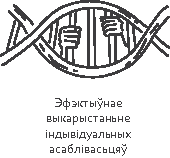
\includegraphics[scale=1.5]{willpower/ch3/1.pdf}
\end{figure}

\textbf{Рызыка для вас тым вышэйшая, чым бліжэйшая ступень сваяцтва, чым больш выпадкаў у~радаводзе, чым ранейшы ўзрост праявы хваробы.}

Запісвайце любую інфармацыю, нават калі на першы погляд яна здаецца непатрэбнай, бо заканамернасьці можна выявіць толькі пры поўнай пабудове ўсяго радавога дрэва здароўя. Акрамя генаў мы ўспадкоўваем і асаблівасьці іх рэгуляцыі (эпігенэтыка), і ўстаноўкі мысьленьня і каштоўнасьці (сацыяльнае ўспадкоўваньне) і, напрыклад, часткова мікрабіём.

Пазьнейшы час пачатку захворваньняў, захаваньне кагнітыўных здольнасьцяў да глыбокай старасьці, высокая працягласьць жыцьця~--- гэта станоўчыя прыкметы, бо супэрдоўгажыхары, як правіла, маюць важны ўклад у~генэтыку.

\subsection*{Пытаньні і заданьні}

1. Якія паказьнікі вы штодня вымяраеце?

2. Што б вам хацелася пачаць вымяраць? У якіх выпадках вы адчуваеце ўнутраны супраціў і адмаўляецеся ад вымярэньняў? Чаму?

3. Зьбярыце сямейную гісторыю здароўя.


\section{Прынцып «што і як вымяраць»}

\emph{Канарэйкі вельмі адчувальныя да дамешкаў шкодных газаў, таму ў~далёкім мінулым шахтары бралі клеткі з~гэтымі маленькімі птушачкамі з~сабой у~шахты. Калі птушка рэзка мяняла паводзіны або гінула, то шахтары тут жа сыходзілі з~гэтага месца~--- і заставаліся жывымі. Такім чынам, забруджанасьць паветра вымяралася канарэйкамі. А як пачуваецца вашая канарэйка?}

У сьвеце сучаснай мэдыцыны існуе велізарная колькасьць параметраў, якія вы можаце вымераць. Калі вы прыйдзеце ў~паліклініку, вам парэкамэндуюць прайсьці цалкам умераны комплекс абсьледаваньняў, у~той час як адэпты руху Quantified Self~--- «вымярэньне сябе», або лайфлогінг,~--- ня проста здымаюць сотні паказьнікаў на працягу доўгага часу, але й аблічбоўваюць іх у~адкрытым доступе на адмысловых сайтах.

Мы можам вымяраць сваю фізычную актыўнасьць (фітнэс-трэкеры), якасьць сну, вагу, целасклад, узровень глюкозы, узровень кетонавых целаў у~выдыханым паветры, кіслотнасьць мачы, электракардыяграфію, варыябельнасьць пульсу, частасьць дыханьня, частасьць сардэчных скарачэньняў, артэрыяльны ціск, цяглічнае напружаньне, электраэнцэфалаграму і гэтак далей. Можна з~дапамогай спэцыяльных праграмаў адзначаць свой узровень шчасьця й энэргічнасьці ў~пэўныя адрэзкі дня і аб'ектыўна вымяраць прагрэс у~мэдытацыі з~дапамогай нэўрагарнітураў накшталт Muse. Ёсьць магчымасьць сабраць даныя ДНК-тэстаў, прааналізаваць мікрабіёту, зазірнуць у~арганізм з~дапамогай МРТ і шмат чаго яшчэ.

\begin{figure}[htb!]
  \centering
  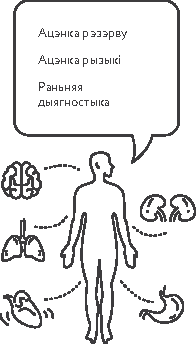
\includegraphics[scale=1.5]{willpower/ch3/2.pdf}
\end{figure}

\emph{Масіў прадукаваных намі зьвестак мы можам успрымаць як своеасаблівае «віртуальнае» люстэрка, як спосаб назіраць за сабой аб'ектыўна, не належачы на эмацыйныя адзнакі.}

Такі спосаб назіраньня дае нам свабоду і магчымасьць рэальна зразумець, што і як працуе ў~нашым целе, бяз возірку на стэрэатыпы і ўсярэдненыя ўяўленьні. Мы можам пазбавіцца ад шматлікіх навязаных нам перакананьняў, асвойваць новыя звычкі ды адчуваньні, захоўваць свой жыцьцёвы досьвед у~лічбавым выглядзе і дзяліцца гэтымі зьвесткамі з~навакольнымі.

Многія нашы станы маюць невідавочныя прычынна-выніковыя сувязі. Напрыклад, што агульнае паміж узроўнем глюкозы ноччу і энэргічнасьцю раніцай? Што лепей~--- трэніроўка да або пасьля яды? Як зразумець, ці сапраўды працуе мэтад рэляксацыі ці вы проста нудзіцеся з~зачыненымі вачамі? Адчуваньне кантролю, якое нараджае назіраньне, таксама вельмі важнае. Мы адчуваем павелічэньне ўласных магчымасьцяў, свой патэнцыял. Пачынаем верыць, што можам зьмяніць свае паводзіны. 

\infobox{Усьведамленьне такой самаэфэктыўнасьці працуе нашмат лепш, чым традыцыйнае запалохваньне нэгатыўнымі наступствамі нездаровага ладу жыцьця. Страх не працуе для абсалютнай большасьці людзей на доўгатэрміновай аснове.}

\subsection*{Вядзеньне дзёньніка}

\textbf{Дзёньнік сну, харчаваньня, узроўню стрэсу, трэніровак, усьвядомленасьці і мэдытацыяў} можна весьці па адной схэме: запісваць задачы, адзначаць аб'ём выкананага, якасьць самаадчуваньня, уносіць ідэі зы заўвагі. Раз на тыдзень, напрыклад, на выходных, прааналізуйце запісы і занатуйце мэты на наступны тыдзень. Раз на месяц праглядайце ўсе чатыры тыдні, адсочваючы прагрэс. Вызначайце, што добрага трэба дадаць, што можна прыбраць, што трэба прыняць. Занатоўвайце высновы і адкрыцьці вашых разважаньняў і тыднёвага аналізу. Можна выкарыстоўваць дзёньнікі як у~папяровым, так і ў~лічбавым варыянце, адсочваючы кожны з~рэсурсаў здароўя або яго асобныя кампанэнты.

\emph{\textbf{Дзёньнік перамогаў, падзякі, задавальненьня і ня толькі.} Даведзена, што любыя перамогі павышаюць узровень тэстастэрону і адчувальнасьць мозгу да яго: адзначаючы свае дасягненьні, вы робіце сабе добра. Ёсьць фармат дзёньніка ўзаемаадносінаў, дзе партнэры ці муж і жонка робяць свае запісы, гэта дапамагае ўзаемаразуменьню і паляпшае адносіны ў~70\,\% выпадкаў. Можна весьці журнал памылак або журнал марнаваньняў часу. Або, напрыклад, паспрабуйце скласьці антырасклад, куды вы першымі пачняце ўносіць адпачынак, час яды, сон, заняткі спортам і ўзнагароды сябе. Так вы зможаце ўзаконіць у~сваім жыцьці заняткі здароўем без пачуцьця віны, бо не выпадкова кажуць, што праца~--- адна з~самых небясьпечных формаў пракрастынацыі.}

\begin{figure}[htb!]
  \centering
  
\includegraphics[scale=1.5]{willpower/ch3/3.pdf}
\end{figure}

\subsection*{Штодзёньнік}

Я выкарыстоўваю клясычны штотыднёвік з~адным разваротам на ўвесь тыдзень, каб бачыць яго цалкам для пастаноўкі галоўных задачаў. Заўсёды побач у~мяне ляжыць працоўны сшытак~--- запісваю туды розныя думкі па ходзе сваёй працы і жыцьці. Таксама выкарыстоўваю маленькія аркушы паперы для розных ідэй, іх потым лёгка адсартаваць па тэматычных праектах. Кожны дзень на аркушык для нататак выпісваю ключавыя мэты дня і трымаю яго перад вачыма як напамін. Раніцай хаця б на пяць хвілінаў разгортваю «журнал асабістага», дзе ўклейваю натхняльныя выявы, цытаты, ідэі, структурую свае каштоўнасьці і пляны, упісваю падзякі, задавальненьні, перамогі. Зразумела, весьці запісы можна і ў~лічбавым варыянце~--- у~Google keep, Evernote і любой іншай зручнай для вас праграме.

\subsection*{Чэк-сьпісы, або кантрольныя сьпісы}

Чэк-сьпіс~--- гэта сьпіс умоваў, якіх трэба прытрымлівацца пры выкананьні задачы. Гэтая тэхніка дазваляе адсочваць якасьць паўсядзённай рутыны і дбайнасьць выкананьня пастаўленых сабе заданьняў. Зь цягам часу нашыя звычкі пачынаюць «дрэйфаваць», мы можам страчваць фокус і пачуцьцё напрамку. Кантрольны сьпіс~--- у~ідэале ён зьмяшчаецца на адным аркушы і дапамагае пільнавацца абранага шляху.

\subsection*{Пытайцеся ў~сябе}

Практыка задаваць сабе пытаньні і шчыра на іх адказваць~--- выдатны інструмэнт. Для гэтага можна выкарыстоўваць чат-боты або праграмы для адказаў на пытаньні. Старайцеся фармуляваць пытаньні так, каб яны актыўна залучалі вас у~разважаньні ды самааналіз. Хоць самае простае, што вы можаце зрабіць, каб ацаніць якасьць вашага жыцьця,~--- перастаньце нешта рабіць і прыслухайцеся, як вы сябе адчуваеце. 

\textbf{Як я магу атрымаць інфармацыю пра гэты аспэкт свайго жыцьця і здароўя? Што азначаюць атрыманыя зьвесткі? Якія магчымасьці я маю? Як мне ўключыць гэта ў~сваё паўсядзённае жыцьцё? Што я зрабіў сёньня, каб добра сябе адчуваць?}

\subsection*{Паказьнікі здароўя й гаджэты}

Чым займаюцца біяхакеры? Вымяраюць сябе, дастасоўваюць да вялікага мноства мэтрыкаў сыстэмны падыход, паляпшаюць «пэрсанальныя зьвесткі», уплываючы як на свой арганізм, так і на навакольнае асяродзьдзе. Біяхакеры выкарыстоўваюць прасунутыя фітнэс-трэкеры (напрыклад, смарт-пярсьцёнак Ourа), якія сочаць за колькасьцю крокаў, варыябэльнасьцю пульсу, фазамі сну і да т.~п. Распаўсюд атрымліваюць прылады дыстанцыйнага маніторынгу здароўя (non-wearable гаджэты), бо насіць і подзаряжать шматлікія гаджэты няёмка. Таму існуе, напрыклад, рэгістрацыя сну сэнсарнай стужкай у~ложку. Зьмяншэньне памераў прыладаў вядзе да павелічэньня хібнасьці вымярэньняў у~параўнаньні зь лябараторнымі вымярэньнямі. Праўда, вытворцы такіх прыладаў запэўніваюць, што розьніца ў~вымярэньні якасьці сну лябараторнай полісамнаграфіяй і фітнэс-бранзалетам складае ня больш за 10\,\%, аднак іншыя зьвесткі гавораць аб значных памылках.

\begin{figure}[htb!]
  \centering
  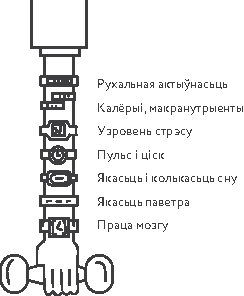
\includegraphics[scale=1.5]{willpower/ch3/4.pdf}
\end{figure}

Мы можам ацэньваць ня толькі ўнутранае, але і навакольнае асяродзьдзе, заўважаючы, як на наша здароўе і самаадчуваньне ўплывае ўсё, што нас атачае. Напрыклад, праграмы SunDay: Vitamin D \& UV Monitor або Dminder дапамогуць адсачыць сонечную актыўнасьць, час для загару і ўзровень вітаміну D. Падключаныя да смартфона датчыкі вуглякіслага газу (CO\textsubscript{2}), чысьціні паветра (P.M 2,5), вільготнасьці ды іншыя дапамагаюць сачыць за якасьцю паветра як унутры пакоя, так і на дварэ.

\subsection*{Біямаркеры}

У XVIII стагодзьдзі лекары наракалі, што «падковам і капытам коней людзі надаюць больш увагі, чым уласным нагам», у~XXI стагодзьдзі людзі часьцяком трацяць больш часу на аўтамабіль або дызайн сваёй кватэры, чым на сваё здароўе. Вядомыя вам біямаркеры дапамагаюць правільна расставіць прыярытэты: даць адзнаку рэальнага стану рэчаў, спрагназаваць, ацаніць рызыкі. Чым вышэйшая рызыка таго ці іншага захворваньня, тым больш агрэсіўнай павінна быць тэрапія, больш дбайным~--- адсочваньне прагрэсу, больш падрабязным~--- маніторынг пабочных эфэктаў і да т.~п.

\emph{Апошнім часам папулярнасьць набываюць «оміксныя» аналізы, калі вывучаецца поўны профіль: аналіз усяго геному, мікрабіёму, эпігеному, транскрыптому (РНК-профіль), цытакіному (набор цытакінаў~--- узровень запаленьня), пратэому (набор бялкоў крыві), мэтабалёма (профіль і канцэнтрацыя нутрыентаў у~крыві) і да т.~п. Але такія падыходы вельмі дарагія і пакуль недасяжныя большасьці чытачоў, хоць па аналізе ДНК мы ўжо сёньня можам падбіраць больш аптымальныя прэпараты (фармакагеноміка). Камбінаванае выкарыстаньне ўсіх «омікаў» для канкрэтнай мэты называецца паноміка («panomics»), і, магчыма, за ёй будучыня прэцызійнай (дакладнай) мэдыцыны, якая дазваляе максімальна дакладна падбіраць лячэньне для канкрэтнага чалавека з~канкрэтнай хваробай.}

Напрыклад, дасьледаваньні паказваюць, што, калі людзі зь пераддыябэтам ня ўносяць карэктываў у~свой лад жыцьця, большасьць зб іх на працягу 10 гадоў сутыкаецца з~разьвіцьцём цукровага дыябэту 2 тыпу, зь іх у~15--30\,\% хвароба разьвіваецца на працягу пяці гадоў. Калі людзі з~пачатковымі кагнітыўнымі разладамі нічога ня робяць, у~іх ёсьць вельмі высокая рызыка разьвіцьця дэменцыі бліжэйшым часам.

Важна адрозьніваць «норму» і «оптымум» для кожнага з~маркераў. Напрыклад, для С-рэактыўнага бялку ў~шматлікіх лябараторыях нормай пазначанае значэньне 5, хоць аптымальнымі зьяўляюцца значэньні 0,1--0,65, а~рызыка для здароўя расьце ўжо са значэньня 1.1. Таксама аптымальнае значэньне залежыць ад канкрэтнай тэрапэўтычнай мэты. Напрыклад, чым вышэйшая рызыка сардэчна-сасудзістых захворваньняў, тым меншым будзе аптымальнае значэньне ЛПНШ (ліпапратэіны нізкае шчыльнасьці).

Мінімальны набор аналізаў уключае такія базавыя паказьнікі, як глюкоза, інсулін, глікаваны гемаглябін, ліпідны профіль, С-рэактыўны бялок, мачавая кіслата, ТТГ, св. тэстастэрон, АлАт, АсАт, білірубін, крэатынін, агульны бялок, агульны аналіз крыві і мачы. Прыклад разгорнутай панэлі біямаркераў прыведзены ніжэй. Для захоўваньня і аналізу вынікаў можна выкарыстоўваць адмысловую праграму, якая было створаная пры маім удзеле,~--- CarrotCare (iOS).

\textbf{Біямаркеры, якія можна маніторыць:}

\begin{figure}[htb!]
  \centering
  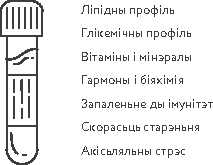
\includegraphics[scale=1.5]{willpower/ch3/5.pdf}
\end{figure}

\emph{\textbf{Глікемічны статус:} глікаваны гемаглабін, інсулін, глюкоза, індэкс інсулінарэзыстэнтнасьці (HOMA-IR).}

\emph{\textbf{Тлушчавы статус:} агульны халестэрын, халестэрын высокай шчыльнасьці, халестэрын нізкай шчыльнасьці, трыгліцэрыды, акісьленыя ЛПНШ, аполіпапратэін А1 аполіпапратэін В, лептын, адыпанэктын, амэга-3 індэкс і вытворныя гэтых паказьнікаў.}

\emph{\textbf{Запаленчыя маркеры:} высокачуллівы тэст на С-рэактыўны бялок, інтэрлейкін 6, фібрынаген.}

\emph{\textbf{Гармоны:} палавыя гармоны: агульны і свабодны тэстастэрон, ГЗПГ, праляктын, эстрадыёл, ДГЭА, ЛГ, ФСГ; гармоны шчытавіцы: ТТГ, свабодныя Т3 і Т4; іншыя гармоны: ІФР-1.}

\emph{\textbf{Пячоначныя маркеры:} альбумін, білірубін агульны і зьвязаны, Алат, Асат, ГГТП.}

\emph{\textbf{Вітаміны:} вітамін D, вітамін B\textsubscript{12} (галатранскабалямін), вітамін B\textsubscript{9}.}

\emph{\textbf{Мінэралы:} жалеза, цынк, магній, ёд, медзь, сэлен, фэрытын, цэруляплязьмін, калій, натрый, кальцый.}

\emph{\textbf{Іншыя паказьнікі:} гомацыстэін, мачавая кіслата, мачавіна, крэатынін, СКФ хуткасьць клубочковой фільтрацыі, агульны аналіз крыві.}

\subsection*{Хатнія прылады}

Цяпер можна купіць розныя датчыкі для самастойнага вымярэньня паказьнікаў здароўя~--- ад узроўню глюкозы і кетонавых целаў у~мачы або дыханьні да ціску і сатурацыі (узровень насычэньня крыві кіслародам). У прыватнасьці, за час распаўсюджваньня каранавіруснай інфэкцыі павысіўся попыт на пульсаксімэтры~--- апараты, якія вызначаюць сатурацыю, каб была магчымасьць своечасова заўважыць дыхальную недастатковасьць.

\emph{Зьявілася шмат датчыкаў для кругласутачнага адсочваньня ваганьняў глюкозы, напрыклад Free Libre. Яны дапамагаюць заўважыць скокі глюкозы ў~здаровых людзей і выявіць іх прычыны. Аказваецца, у~розных людзей бываюць розныя глюкатыпы са сваёй амплітудай ваганьняў узроўняў глюкозы. Маніторынг таксама дазваляе выявіць індывідуальную глікемічную рэакцыю на прадукты, убачыць эпізоды як гіпэрглікеміі, так і ўтоенай гіпаглікеміі і зьвязаць іх з~пэўнымі станамі. Празьмерны і працяглы скачок глюкозы пасьля прыёму ежы павышае рызыку інфаркту міякарда ў~4--5 разоў, прычым незалежна ад яе ўзроўню нашча. З дапамогай аптэчнага аналізатара ўзроўню глюкозы можна вымяраць рэакцыю менавіта на прыём ежы.}

\subsection*{Інструмэнтальныя вымярэньні}

Бадай кожны орган можа быць старанна абсьледаваны~--- і для гэтага вынайшлі мноства розных мэдыцынскіх спосабаў абсьледаваньня. Напрыклад, ацэнка стану сардэчна-сасудзістай сыстэмы ўключае вымярэньне артэрыяльнага ціску, пульсу спакою, УГД сасудаў шыі, УГД міякарда, мультысьпіральную кампутарную тамаграфію сасудаў сэрца, вымярэньне калянасьці артэрыяў рознымі спосабамі, ЭКГ, манжэтавы тэст, нагрузачныя тэсты. Мэтазгоднасьць выбару таго ці іншага інструмэнту залежыць ад канкрэтнае сытуацыі.

\textbf{Напрыклад, якія ёсьць дасьледаваньні сэрца і сасудаў?}

\emph{\textbf{Ультрагукавыя дасьледаваньні.} УГД брахіяцэфальных сасудаў з~вызначэньнем таўшчыні комплексу інтыма-мэдыя. Таўшчыня комплексу інтыма-мэдыя~--- гэта важны паказьнік рызыкі атэрасклерозу і гіпэртрафіі цяглічнага пласта сасудаў. Таксама такое абсьледаваньне выяўляе наяўнасьць або адсутнасьць атэрасклератычных бляшак, што паказвае іх распаўсюджанасьць і ў~іншых сасудах арганізма. Кожны 0,1 мм таўшчыні павялічвае рызыку інфаркту міякарда на 15\,\%. Значэньні вышэйшыя за 0,9 мм лічацца высокімі, нармальныя значэньні~--- 0,7 мм і ніжэй.}

\emph{\textbf{Эхакардыяграфія.} ЭхаКГ сэрца зьяўляецца адчувальным мэтадам дасьледаваньня стану міякарду. Карысны і «манжэтавы» тэст, ён жа «крываток-апасродкаванае пашырэньне» (FMD~--- Flow Mediated Dilatation) плечавай артэрыі, калі яе перакрываюць манжэтай на 5 хвілінаў, а~затым, пасьля зьняцьця, ацэньваюць прырост дыямэтра плечавай артэрыі~--- слабы прырост гаворыць пра эндатэліяльную дысфункцыю.}

\emph{\textbf{ЭКГ.} Паколькі часам небясьпека тоіцца ў~парушэньнях рытму, то абавязкова трэба праводзіць содневы маніторынг ЭКГ Холтэра, якіе нярэдка фіксуе арытміі, ня бачныя на звычайнай кардыяграме. Нагрузачная проба (трэдміл або велаэргамэтрыя) дазваляе ацаніць, як рэагуе ЭКГ на павелічэньне частасьці сардэчных скарачэньняў, ці зьяўляюцца ішэмічныя зьмены, парушэньні рытму, ці падвышаецца ціск.}

\begin{figure}[htb!]
  \centering
  
\includegraphics[scale=1.5]{willpower/ch3/6.pdf}
\end{figure}

\emph{\textbf{Мультысьпіральная кампутарная тамаграфія сасудаў сэрца} паказвае адклады кальцыю ў~сасудах сэрца, што дастаткова дакладна вызначае вашую рызыку. Колькасьць кальцыя вымяраецца ў~кальцыевым індэксе паводле Агатстона. Ідэальнае значэньне нуль, але каранарная кальцыфікацыя вышэйшая за 300 адзінак Агатстона~--- гэта паказьнік высокай рызыкі.}

\emph{\textbf{Калянасьць артэрыяў.} Калянасьць сасудзістай сьценкі звычайна вызначаецца з~выкарыстаньнем вымярэньня хуткасьці распаўсюджваньня пульсавай хвалі ў~аорце або аартальнага індэксу аугмэнтацыі. Падвышаная калянасьць зьяўляецца чыньнікам рызыкі сардэчна-сасудзістых захворваньняў. Вымераць яе можна адмысловымі прыладамі, а~ўскосна меркаваць пра яе~--- па шчыкалатка-плечавым індэксе (ШПІ) і пульсавым ціску.}

Ідэя шматлікіх вымярэньняў выглядае выдатнай, аднак тут ёсьць шэраг слабых месцаў. Якіх?

\subsection*{Дакладнасьць вымярэньняў}

У адным з~дасьледаваньняў удзельнікі апраналі на адну руку некалькі фітнэс-бранзалетаў і атрымлівалі выразна адрозныя значэньні актыўнасьці. Таму важна правяраць дакладнасьць, сачыць за трэндамі зьвестак, то бок за дынамікай ваганьняў працяглы час. Гэта дазволіць адрозьніць выпадковае ад заканамернага.

\subsection*{Самаацэнка}

Важна пазьбягаць нэгатыўнай ацэнкі сваіх намаганьняў і параўнаньня сябе зь іншымі. Дасьледаваньні паказваюць: калі вы лічыце, што ваша актыўнасьць горшая, чым у~знаёмых, то імавернасьць таго, што вы зоймецеся спортам, зьніжаецца! Людзі, якія лічаць, што займаюцца спортам больш за сваіх сяброў, жывуць даўжэй, нягледзячы на аднолькавы аб'ём трэніровак і аднолькавы ўзровень здароўя. Таму ня трэба параўноўваць сябе з~рознымі спартоўцамі ў~фэйсбуку і хвалявацца. Занадта сур'ёзнае і крытычнае стаўленьне да свайго здароўя і канцэнтрацыя на нэгатыве можа прывесьці да эфэкту нацэба (антыплацэба), што правакуе нездароўе. Не параўноўвайце сябе зь іншымі і стаўцеся з~аптымізмам нават да невялікіх сваіх крокаў!

\subsection*{Марнаваньне часу}

Вымярэньне мноства паказьнікаў зьядае час. Бо рэсурс нашай увагі абмежаваны, мы можам губляць шмат часу на рутыну, а~працаздольнасьць пры гэтым будзе зьмяншацца. Дасьледаваньні паказваюць, што гаджэты не заўсёды аказваюць такі ж пазітыўны ўплыў, як, напрыклад, вядзеньне дзёньніка. Хаця тыя, хто насіў фітнэс-бранзалет, прысьвячалі фізычнай актыўнасьці ў~тыдзень на паўгадзіны больш, розьніцы ў~здароўі паміж удзельнікамі кантрольнай групы выяўлена не было. Іншае дасьледаваньне паказала, што тыя, хто не насіў гаджэт, у~праграме пахуданьня скінулі больш вагі.

\subsection*{Закон Гудхарта}

«Любая назіраная статыстычная заканамернасьць схільная да разбурэньня, як толькі на яе аказваецца ціск з~мэтай кіраваньня». Гэтае правіла з~эканомікі абвяшчае: калі мы ставім сабе мэтай дасягнуць нейкі паказьнік, то ранейшыя заканамернасьці, якія яго выкарыстоўваюць, перастаюць працаваць. \textbf{Інакш гэтае правіла можна сфармуляваць так: «Калі нейкі паказьнік становіцца мэтай, ён перастае быць добрым паказьнікам».}

\emph{Калі арыентавацца на адзін паказьнік, ігнаруючы астатнія, гэта, хутчэй за ўсё, прывядзе да памылак. Нельга ацэньваць стан машыны па прабегу (лічыльнік лёгка скруціць), ня варта ацэньваць каханьне па колькасьці падарункаў, а~дзяцей~--- па прынесеных ацэнках. Біямаркеры~--- гэта добра, але яны павінны быць толькі падказкамі, а~ня нашымі мэтамі. Напрыклад, эпігенэтычны ўзрост можна адкаціць вітамінам Д, гармонам росту, вітамінамі B\textsubscript{9} і B\textsubscript{12}, шэрагам прадуктаў (мяса птушкі), але ніводнае з~гэтых умяшаньняў не зьмяншае сьмяротнасьць і не падаўжае жыцьцё.}

Заўсёды важна трымаць фокус на «цьвёрдых» канчатковых пунктах. Калі мы ставім мэты ці ацэньваем прагрэс, вельмі карысна памятаць пра правіла Гудхарта, каб ня зьбіцца са шляху.

\subsection*{Гіпэрдыягностыка}

Гэта дастаткова небясьпечная зьява ў~сучаснай мэдыцыне, нароўні з~залішнім лячэньнем. Абсьледаваньне здаровых людзей часта вядзе да пастаноўкі непатрэбных дыягназаў. Гэта чапляе на чалавека пэўны цэтлік і прыводзіць да таго, што шматлікія яго сымптомы спрабуюць растлумачыць ужо пастаўленым дыягназам. Такі чалавек атрымлівае непатрэбнае лячэньне і праходзіць празь непатрэбныя працэдуры, хоць ён пры гэтым здаровы ці мае мінімальную рызыку. Вельмі часта даводзіцца супакойваць запалоханых шматлікімі дыягназамі людзей.

Дарога ў~пекла выбрукаваная добрымі намерамі, і часам жаданьне дапамагчы вядзе да неспрыяльных наступстваў. Псэўдазахворваньне~--- гэта выяўленьне такіх формаў хваробы, якія ніколі б не прывялі да зьяўленьня сымптомаў або заўчаснай сьмерці.

\emph{Паводле дасьледаваньняў, каля траціны людзей з~дыягназам «астма» ня маюць такога захворваньня, а~дыягназ «гіпэртэнзія» часам можа быць пастаўлены няслушна: гіпэртэнізія «белага халата»~--- сам факт наведваньня лекара ў~паліклініцы прыводзіць да павышэньня ціску. Або, напрыклад, падвышэньне антыцелаў да шчытавіцы для некаторых адмыслоўцаў ужо зьяўляецца нагодай для ўмяшаньня. Такім жа чынам часта ставяцца неабгрунтаваныя псыхіятрычныя дыягназы, астэахандроз, СДУГ і нават рак.}

\emph{Пры поўным МРТ цела ў~40\,\% людзей могуць быць выяўленыя нейкія ўтварэньні, якія называюць «інцэдалома». У абсалютнай большасьці выпадкаў гэта дабраякасныя ўтварэньні, напрыклад гемангіёмы печані. Калі кожнае з~такіх утварэньняў пункціраваць або спрабаваць выдаліць, гэта можа нанесьці сур'ёзную шкоду здароўю.}

Вядома, тут працуе і праблема чаканьняў: калі ўжо нешта выяўлена, то ад лекара чакаюць прызначэньня разгорнутага лячэньня, а~ня проста назіраньня або парадаў па зьмене ладу жыцьця. І заўсёды застаецца пытаньне асабістай карысьці: калі ў~сярэднім нейкі спосаб раньняй дыягностыкі можа быць неэфэктыўным, то менавіта ў~вашым выпадку ён можа выратаваць жыцьцё.

\subsection*{Індывідуальная праграма}

Канкрэтная праграма абсьледаваньняў залежыць ад узросту чалавека, наяўнасьці чыньнікаў рызыкі захворваньняў, біямаркераў. Напрыклад, для вызначэньня аптымальнага спосабу скрынінгу каларэктальнага раку важна ведаць, што яго чыньнікамі рызыкі зьяўляюцца запаленчыя захворваньні кішачніка (язвавы каліт, хвароба Крона), спадчынны адэнаматозны паліпоз, пэўны стыль харчаваньня. Таксама наяўнасьць сваякоў з~каларэктальным ракам павышае рызыку ў~2--3 разы: калі ў~іх быў рак ва ўзросьце да 60 гадоў, то трэба пачынаць скрынінг у~45 гадоў~--- за 15 гадоў да. Як мінімум мне б хацелася, каб у~вас быў свой выразны плян здароўя на год і на 10 гадоў наперад. \textbf{Вялікая колькасьць чыньнікаў рызыкі якога-небудзь захворваньня патрабуе больш дбайнай і раньняй прафіляктыкі.}

\infobox{Зьбярыце інфармацыю пра сваё здароўе ў~адным месцы, магчыма, і на воблачным носьбіце, бо ўсе выпіскі на паперы губляюцца. Разглядайце здароўе ў~шырокім ключы: гэта і рызыка ДТЗ, фінансавыя рызыкі, рызыкі залежнасьці, суіцыду, прафіляктычныя мерапрыемствы, уключаючы прышчэпкі ня толькі для дзяцей, але і для дарослых, маніторынг пабочных эфэктаў лекаў.}

\textbf{Раньняя дыягностыка.} \emph{«Мудрыя лячылі сябе раней, чым выяўлялася захворваньне... Чакаць хваробу, каб ужываць лекі, ці чакаць парушэньні, каб затым дамагацца супакою,~--- гэта ўсё роўна як, дачакаўшыся смагі, пачаць капаць калодзеж, ці дачакацца пачатку вайны, каб каваць зброю. Ці ня будзе занадта позна?»} (Нэй-Цзін).

Прафіляктычныя дасьледаваньні мае сэнс пачынаць прыкметна раней, чым рэкамэндуюць. Так, атэрасклератычнае паражэньне сасудаў пачынаецца рана ў~жыцьці, але прагрэсуе з~рознай хуткасьцю. У многіх назіраецца паскораны атэрасклероз, які клінічна значны ўжо ў~маладым узросьце. Пагатоў тыповыя чыньнікі рызыкі не заўсёды прадказваюць яго. А 80\,\% выпадкаў раптоўнае каранарнае сьмерці зьвязана з~атэрасклерозам.

Дасьледаваньне PDAY вывучала аўтапсіі амаль 3000 людзей ва ўзросьце 15--34, 13\,\% абсьледаваных аказаліся з~выяўленым атэрасклерозам (уключна зь нестабільнымі бляшкамі). Выяўленыя прыкметы атэрасклерозу абдамінальнай аорты ў~20\,\% (15--19 гадоў), 40\,\% (30--34 гады), паражэньне каранарных артэрыяў у~10\,\% (15--19 гадоў), 30\,\% (30--34 гады). У іншым дасьледаваньні УГД паказала прыкметы каранарнага атэрасклерозу ў~15\,\% людзей маладзейшых за 20, 37\,\% ва ўзросьце 20--29, 60\,\% ва ўзросьце 30--39, 71\,\% ва ўзросьце 40--49, 85\,\% ва ўзросьце старэйшых за 50. Аўтапсіі загінулых жаўнераў (сярэдні ўзрост 26) паказалі каранарны атэрасклероз у~78\,\%, пры гэтым звужэньне прасьвету артэрыяў больш чым на 50\,\%~--- у~20\,\% выпадкаў, больш за 75\,\% прасьвету~--- у~9\,\%. Як бачыце, паражэньні сардэчна-сасудзістай сыстэмы часта ўзьнікаюць даволі рана. Таму прэвэнтыўная дыягностыка можа быць эфэктыўнай і карыснай. Можна запаволіць і нават скіраваць назад працэс атэрасклерозу.

\emph{\textbf{Генэтычнае тэставаньне.} Існуе вялікая колькасьць розных тэхналёгіяў тэставаньня, ад частковага да поўнагеномнага, і кампаніяў, якія займаюцца тэставаньнем. Варта загадзя адзначыць, што сувязь захворваньне--гены далёка не заўсёды адназначная, таму да атрыманых рэкамэндацыяў варта ставіцца скептычна.}

\begin{figure}[htb!]
  \centering
  
\includegraphics[scale=1.5]{willpower/ch3/7.pdf}
\end{figure}

\textbf{Толькі невялікая колькасьць генаў вывучаная настолькі, што стала магчымым вызначыць іх узаемасувязь зь некаторымі захворваньнямі і спосабы перадухіленьня рызыкі. Напрыклад, сувязь BRCA1 і раку грудзей, APOE і хваробы Альцгаймэра.}

\emph{Што тычыцца мультыфактарыяльных захворваньняў, напрыклад атлусьценьня, то дакладнасьць генэтычнага тэставаньня тут дастаткова малая і можа перакрывацца асяродзьдзем і ладам жыцьця. Нязначнае павелічэньне рызыкі, як правіла, не нясе практычнай інфармацыі і не вястуе ўзьнікненьня захворваньня. Таму для шматлікіх хваробаў лябараторны аналіз крыві куды дакладнейшы за генэтычны тэст. Гэтую паслугу прапануюць розныя кампаніі, ад 23andMe да расшыфроўкі поўнага геному па ўмераных коштах у~Dante Labs.}

\emph{Многія гены дазваляюць ацаніць нашу рэакцыю на розныя прадукты і лекавыя прэпараты: напрыклад, у~каго кафэін выклікае трывожнасьць або артэрыяльную гіпэртэнзію, у~каго вышэйшая рызыка пабочных эфэктаў пры ўжываньні пэўных прэпаратаў, для каго гэтыя лекі будуць асабліва эфэктыўныя ці неэфэктыўныя. Можна ацаніць свае спартовыя здольнасьці (напрыклад, маратонец вы ці спрынтар), даведацца пра ўнікальныя характарыстыкі, пачынаючы ад успрыманьня пахаў і смакаў да вызначэньня хранатыпу (сава ці жаўрук). Выбар жа пэўнай дыеты ці віяду спорту паводле зьвестак тэсту пакуль не атрымаў дастатковай колькасьці навуковых пацьверджаньняў.}

\subsection*{Пытаньні і заданьні}

1. Ці робіце вы штогадовае абсьледаваньне?

2. Ці ёсьць у~вас індывідуальная праграма абсьледаваньня? Ці ведаеце вы свае рызыкі?

3. Ці часта вы турбуецеся праз вынікі абсьледаваньня?


\section{Прынцып «прасьцей, не ўскладняйце»}

«Колькі здароўя і сіл змарнаваў на сваё здароўе і сілу» (О'Генры). Калі людзі заканчваюць мае навучальныя курсы рэсурсаў здароўя, то дзівяцца, як складана створаныя наша цела і мозг і як проста весьці здаровы лад жыцьця. Пачуцьцё яснасьці і палёгка~--- гэта натхняльныя азарэньні. Бо сучасныя мэдыя прапануюць такі набор узаемна супрацьлеглых поглядаў на здароўе, што чалавек блытаецца, нявызначанасьць замінае яму дзейнічаць правільна.

\textbf{Нашкодзіўшы сабе экстрэмальным аздараўленьнем, чалавек губляе і веру ў~сябе, і ўсякае жаданьне займацца здароўем.} Таму не сьпяшайцеся. Спачатку~--- тэхніка бясьпекі. Бо чым эфэктыўнейшы які-небудзь падыход, тым небясьпечнейшыя могуць быць яго пабочныя эфэкты, а~цалкам бясьпечныя толькі бясплённыя сродкі. Зьмена харчаваньня, павелічэньне нагрузкі, уплыў на сваё асяродзьдзе~--- на кожным кроку можа нешта здарыцца: напрыклад, пры няправільнай тэхніцы практыкаваньняў магчымая траўма, хуткі скід вагі можа толькі справакаваць яе набор.

\textbf{Наш мозг супраціўляецца рэзкім зьменам ладу жыцьця, асабліва калі іх мэта яму да канца незразумелая.} \emph{Чалавек, які еў мала клятчаткі, пры пераходзе на здаровае харчаваньне і рэзкім павелічэньні колькасьці зеляніны, сырой гародніны і бабовых можа сутыкнуцца з~павелічэньнем газаўтварэньня ў~кішачніку. Пакутуючы ад такога пабочнага эфэкту, ён можа вырашыць, што здаровае харчаваньне~--- сапраўды не для яго. Адыліж дастаткова было дзейнічаць паступова, даўшы магчымасьць сваёй мікрафлёры адаптавацца да павелічэньня клятчаткі. Дасьледаваньні паказваюць, што за месяц рэгулярнага ўжываньня абсалютная большасьць выдатна пачынае страваваць і гародніну, і бабовыя. Рухаемся ад невялікай колькасьці тэрмічна апрацаванай гародніны, павялічваем аб'ём, затым дадаём болей сырой~--- дзейнічаем плыўна і пазьбягаем такіх пабочак.}

У шмат каго здаровы лад жыцьця асацыюецца з~чалавекам, які абчапляўся датчыкамі, пастаянна лічыць калёрыі і нэрвова ўвечары ходзіць кругамі, дабіраючы крокі да запаветных 10.000. Калі мы глядзім на свой шчыльны расклад, то адчуваем роспач, бо не знаходзім магчымасьці ўпіхнуць усе гэтыя аздараўленчыя практыкі. 

\infobox{Ня варта хвалявацца. Адказна заяўляю: сапраўдная практыка здароўя павінна зараджаць вас энэргіяй і вызваляць час. Нам патрэбнае здароўе для жыцьця, а~не жыцьцё для здароўя.}

Напрыклад, у~харчаваньні вы зэканоміце кучу часу і сілаў, калі будзеце есьці радзей, 2--3 разы на дзень. Прыбіраючы вячэры, вы вызваліце вячэрні час для адпачынку і камунікацыі. Пазбаўляючыся ад шкодных звычак, будзеце атрымліваць ня толькі прыбаўку здароўя, але й выйгрыш у~часе і энэргіі. Скарачэньне часу, які вы праводзіце ў~сацсетках ці за праглядам сэрыялаў, таксама дадасьць і адпачынку, і бадзёрасьці. 

Сапраўдныя здаровыя звычкі~--- гэта інвэстыцыі, якія шматкроць акупляюцца. Галоўнае, што вам спатрэбіцца,~--- гэта некаторыя намаганьні на этапе іх укараненьня ў~сваё жыцьцё. Працуючы зь людзьмі, я звычайна стараюся нават стрымліваць іх энтузіязм на першым этапе і факусаваць увагу на невялікай колькасьці сапраўды важных рэчаў.

\subsection*{Рабіце менш і заўжды памятайце пра істотнае}

Многія людзі захапляюцца рознымі мэтодыкамі і часта выпускаюць мэту з-пад увагі. Напрыклад, у~харчаваньні пачынаюць факусавацца толькі на «натуральнасьці» прадуктаў, ядучы супэркалярыйныя «натуральныя» сушаныя фінікі, забыўшыся аб правіле кіраваньня калярыйнасьцю. Так, вам падабаецца трэнажор для прапампоўкі асобных пучкоў цягліцаў, які выглядае крута, але для вас нашмат важнейшыя базавыя практыкаваньні. Ня трэба спачатку факусавацца на дэталях, факусуйцеся на галоўным і рабіце яго прасьцейшым. Дасьведчаны кухар скарачае колькасьць страваў у~мэню, каб зрабіць іх ідэальнымі, дасьведчаны трэнер не дае пачаткоўцу дзесяць складаных практыкаваньняў.

\emph{Сфакусуйцеся на тым, што ня будзе мяняцца ў~далейшым, на тым, што важна і эфэктыўна, і заўсёды шукайце лягчэйшы спосаб нешта зрабіць.}

Наколькі акупляюцца інвэстыцыі ў~здароўе? 14 гадоў жыцьця~--- гэта дастатковы выйгрыш для вас? А спалучэньне такіх элемэнтарных правілаў, як адмова ад курэньня, здаровае харчаваньне, падтрыманьне нармальнай структуры цела, зьніжэньне спажываньня алькаголю і паўгадзіны фізычнай актыўнасьці ў~дзень могуць падоўжыць жыцьцё на 14 гадоў у~жанчынаў і на 12 гадоў у~мужчынаў, а~таксама зьнізіць на 55\,\% рызыку сьмерці ад усіх прычынаў, у~тым ліку 44\,\% рызыкі сьмерці ад раку і 72\,\% рызыкі сьмерці ад сардэчна-сасудзістых захворваньняў у~параўнаньні з~тымі, хто не выконвае гэтыя правілы. Няўжо гэтыя пяць правілаў складаныя для выкананьня і патрабуюць адмысловых ведаў? Не. У наступных разьдзелах вы знойдзеце канкрэтныя парады і пратаколы для іх укараненьня ў~паўсядзённае жыцьцё.

\subsection*{Разьвязвайце свае праблемы па меры іх ўплыву на працягласьць жыцьця}

З мадыфікаваных чыньнікаў рызыкі сьмерці, тых, што можна зьмяніць і пазьбегнуць, лепш за ўсё вывучана курэньне. Але ёсьць шэраг іншых чыньнікаў, шкода ад якіх выяўленая ня менш~--- а~часам і мацней, хоць гучаць яны цалкам штодзённа і бясьпечна. Памятайце, асноўную ўвагу трэба надаваць таму, што сапраўды важна, а~ня проста «карысна для здароўя». Карысных рэчаў~--- вялікае мноства, а~жыцьцёва важных насамрэч усяго сем. 

\infobox{Звычкі, якія могуць уплываць на здароўе нават горш за курэньне: гіпадынамія, дрэннае харчаваньне, пустэльніцтва, недасып, стрэс, самота, нізкі сацыяльны статус.}

\textbf{Гіпадынамія.} «Сядзеньне~--- гэта новае курэньне»~--- такія загалоўкі прыцягваюць нашу ўвагу. Сядзячы лад жыцьця больш за 10--12 гадзінаў у~дзень можа выклікаць вялікія праблемы са здароўем. Пры гэтым фітнэс-трэніроўкі 2--3 разы на тыдзень не кампэнсуюць цэлы дзень, праведзены седзячы. Працуйце хоць часткова стоячы, сам так раблю і іншым раю.

\textbf{Дрэннае харчаваньне.} Дрэннае харчаваньне~--- магутны чыньнік рызыкі: па розных ацэнках, харчаваньне складае каля 50\,\% якасьці жыцьця: яно ўплывае на здароўе мацней, чым курэньне, наркотыкі, неабаронены сэкс і шматлікае іншае разам узятае. Зрэшты, гэта ня значыць, што, калі вы ясьце правільна, то вам можна курыць і займацца выпадковым сэксам.

\textbf{Дэфіцыт сонечнага сьвятла.} Пустэльнасьць і пазьбяганьне сонца пагаршае здароўе. Вядома, сонечныя апёкі і салярыі~--- гэта чыньнік рызыкі ўзьнікненьня раку, але дэфіцыт сонечнага сьвятла адмоўна ўплывае на самаадчуваньне.

\textbf{Недасып.} Недасып і зьвязаныя зь ім прычыны сур'ёзна кароцяць працягласьць жыцьця і зьвязаныя з~павелічэньнем рызыкі мноства захворваньняў. Пастаянны недасып горшы за курэньне: ён у~чатыры разы павышае рызыку ўзьнікненьня інсульту і ў~два разы~--- рызыку інфаркту.

\textbf{Стрэс.} Ня ўсякі стрэс кепскі, але некантралюемы хранічны стрэс вельмі небясьпечны. Калі казаць пра «дозу», то хранічны стрэс параўноўваюць з~эквівалентам выкурваньня 5 цыгарэтаў у~дзень. Працагалізм таксама небясьпечны: перапрацоўкі павышаюць рызыку заўчаснае сьмерці на 20\,\%.

\textbf{Самота.} Сацыяльнае асяродзьдзе вельмі важнае для паўнавартаснага здароўя. Паталягічную ізаляцыю і вымушаную самоту параўноўваюць з~курэньнем 15 цыгарэтаў у~дзень і павелічэньнем рызыкі шматлікіх захворваньняў і дэструктыўных паводзінаў. Самота павялічвае рызыку сьмерці ва ўзросьце да 35 гадоў на 30 працэнтаў. Вядома, важна адрозьніваць самоту сьвядомую, якая прыносіць вам задавальненьне, і вымушаную, калі вы пакутуеце ад дэфіцыту камунікацыі.

\textbf{Беднасьць, нізкі сацыяльны статус і няроўнасьць.} Ня верце, што высокая пасада, шматгадовая адукацыя або вялікі даход вам нашкодзяць, усё наадварот. Чым вышэйшую сацыяльную пазыцыю вы займаеце, тым лепшае ваша самаадчуваньне. Чым больш вы зарабляеце, тым даўжэй пражывяце. Чым вы больш пасьпяховыя~--- тым здаравейшыя. Ня верыце? Чытайце разьдзел пра сацыяльны статус.

\subsection*{Прэч пэрфэкцыянізм}

Лепей зрабіць зусім мала, чым наогул нічога: трымайцеся прынцыпу мінімуму. У нас часта жыве памылка~--- прывітаньне пэрфэкцыяністам,~--- што калі ўжо няма магчымасьці зрабіць ідэальна, то ня варта і пачынаць. Але ў~адносінах да здароўя гэта не працуе. 

\infobox{Для падтрыманьня здаровых звычак нават мінімум намаганьняў дапамагае ўтрымліваць сыстэму і не перарываць штодзённы ланцужок дзеяньняў.}

\emph{Зрабіць мінімум~--- не выклікае ўнутранага адрыньваньня, нягледзячы нават на стомленасьць, бо сьмешна ж баяцца 20 прысяданьняў? Няма часу і месца мэдытаваць? Можна выйсьці на гаўбец ці адысьці ў~прыбіральню, каб на працягу пары хвілінаў сфакусавацца на дыханьні. Няма часу на трэніроўку? Прайдзіцеся сходамі: трошкі фізычнай актыўнасьці нашмат лепш, чым наогул ніякага руху.}

\begin{figure}[htb!]
  \centering
  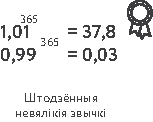
\includegraphics[scale=1.5]{willpower/ch3/8.pdf}
\end{figure}

Першыя крокі~--- найважнейшыя. Найцяжэй нам менавіта пачаць нешта рабіць, ініцыяваць само дзеяньне. Затое ўжо калі пачалі, тут надыходзіць прыемнасьць, і мы ўжо можам займацца даўжэй. Так што як ня хочаце бегаць~--- проста абуйце красоўкі і абыдзіце дом, хай гэта будзе ваш мінімум. Самае нязначнае дзеяньне лепшае за поўную адсутнасьць такога. Напрыклад, калі ў~вас няма часу на перапынак, хоць проста ўстаньце-сядзьце, гэта ўжо будзе добра.

У стрэсавых умовах вельмі карысна любое актыўнае дзеяньне, нават імпульсіўнае~--- а~пры стрэсе мы звычайна дзейнічаем імпульсіўна. Гэта павялічвае адаптыўнасьць, памяншае імавернасьць фармаваньня вывучанай бездапаможнасьці, павялічвае ўпэўненасьць, дапамагае ўкараняць і падтрымліваць звычку ў~новых умовах, у~новым кантэксьце.

\subsection*{Пытаньні і заданьні}

1. Якая асаблівасьць вашага ладу жыцьця, на ваш погляд, мацней за ўсё кароціць яго? Што вы можаце з~гэтым зрабіць?

2. Ці важна вам разумець сэнс рэкамэндацыі па здароўі, каб яе прытрымлівацца?

3. Ці бывала такое, што вы не трымаліся парады, калі яна была заскладаная?


\section{Прынцып «залатой сярэдзіны»}

Жаданьне быць здаровым~--- гэта выдатна, бо «той, хто хоча быць здаровым, збольшага ўжо крыяе». Але многім людзям мала проста акрыяньня, яны хочуць атрымаць усё і адразу: калі ўжо худнець, то жорсткая галадоўка, калі ўжо бегаць, то адразу на маратон, калі ўжо сьвядомасьць, то ў~Індыю на віпасану. Толькі вось жыцьцё~--- гэта маратон, а~ня спрынт, і для бясьпечнай зьмены патрэбны час. Мы забываем, што нашае цела мае свае законы і сваю скорасьць зьмены: цела павольнейшае за розум.

Чым меншая скорасьць~--- тым меншая рызыка зрыву. Важна паступова павялічваць нагрузку, паэтапна скідаць вагу. Напрыклад, бясьпечная хуткасьць пахуданьня вар'юецца ў~значэньнях 500--1000 грамаў на тыдзень. Чым больш чалавек губляе вагі, тым вышэйшая рызыка адкату і ўскладненьняў~--- ад парушэньня харчовых паводзінаў да тлушчавага гепатозу печані.

\textbf{Залатая сярэдзіна здароўя~---} гэта балянс паміж адсутнасьцю якога-небудзь клопату пра здароўе і апантанасьцю ім. Прынцып «больш~--- значыць лепш» тут не працуе. Практычна для ўсіх рэсурсаў здароўя існуе U-падобная сувязь паміж колькасьцю намаганьняў і атрыманай карысьцю. Гэта значыць, што больш~--- гэта часьцяком шкода. Напрыклад, дасьледаваньні выявілі U-падобную сувязь паміж бегам і сьмяротнасьцю: ёсьць верхняя мяжа карысьці і фізычнай актыўнасьці. Залішняя актыўнасьць можа зьмяншаць узровень тэстастэрону, парушаць мэнструальны цыкль, прыгнятаць імунітэт.

\begin{figure}[htb!]
  \centering
  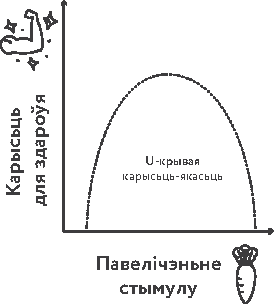
\includegraphics[scale=1.5]{willpower/ch3/9.pdf}
\end{figure}

\emph{\textbf{Здароўе}~--- гэта так крута, ажно можа выклікаць устойлівую залежнасьць, якая патрабавацьме павелічэньня дозы для большага задавальненьня. Рацыянальнасьць тады адсоўваецца на другі плян, галоўнае~--- атрымаць больш кайфу. Таму людзі бягуць усё большыя маратоны, плывуць бясконцыя дыстанцыі, спрабуюць усё даўжэй галадаць, імкнуцца браць усё большую вагу, зьвяртаюцца да рызыкоўных відаў спорту, нягледзячы на высокі траўматызм і рызыку сьмерці. Такія ЗЛЖ-залежнасьці ня маюць нічога агульнага са здароўем. Чалавек, які «зьняўся» з~наркотыкаў і «перасеў» на маратоны, толькі зьмяніў аб'ект залежнасьці, а~не акрыяў. Хоць грамадзкая шкода ад марафонаў, вядома, меншая, чым ад наркотыкаў.}

\textbf{Зашмат карыснага~--- шкодна.} Напрыклад, фолевая кіслата. У высокіх дозах яна ўзмацняе праліфэрацыю клетак, што можа паскорыць атэрасклероз. І калі прадукты забясьпечваюць вам дастатковую колькасьць B\textsubscript{9}, то дадатковы прыём фолію не дадасьць карысьці, але можа павялічыць рызыку для здароўя. Гэта ж датычыцца і вітамінаў, проста прапіваць іх можа быць небясьпечна. Індывідуальны падыход~--- выяўленьне дэфіцытаў і карэкцыя іх. Дэфіцыты могуць узьнікаць з~розных прычынаў~--- нізкае ўтрыманьне вітамінаў або мінэралаў у~прадуктах (кепскі рацыён, бедная глеба), дрэннае ўсмоктваньне праз спалучэньне прадуктаў або захворваньняў (нізкая кіслотнасьць страўніка), генэтычныя асаблівасьці, якія перашкаджаюць засваеньню, падвышанае выдаткаваньне арганізмам. Таксама шкодная залішняя колькасьць вітамінаў B\textsubscript{12}, А, Е і шэрагу іншых. Гіпэрдозы вітаміну D могуць справакаваць кальцыфікацыю крывяносных сасудаў.

Напрыклад, пагаршаюць усмоктваньне жалеза з~прадуктаў і дадаткаў (танін гарбаты, какава, кава і інш.), фітаты (кашы, перапечкі і да т.~п.), фасфаты і кальцый (уся малочка), аксаляты і інш. Так, дадатковы прыём на працягу 10 дзён малака і сыра на 30--50\,\% зьнізіў засваеньне жалеза. А гарбата на 62\,\% зьніжае засваеньне жалеза ў~параўнаньні з~вадой. Паляпшаюць усмоктваньне жалеза: вітамін С ды іншыя арганічныя кіслоты, уключаючы цытрынавую, бурштынавую і інш., фруктоза, сарбіт, амінакіслоты (мэтыянін, цыстэін і інш.), «чыньнік жывёльнага бялку»: міяглабін + гемаглабін. Вітамін С~--- наймацнейшы чыньнік паляпшэньня ўсмоктваньня жалеза. Могуць нашкодзіць і дадаткі, напрыклад п'яце шмат цынку~--- ён блякуе засваеньне медзі, п'яце кальцый~--- ён зьніжае ўсмоктваньне жалеза.

\textbf{Усё залежыць ад дозы і спосабу выкарыстаньня.} Як казаў сярэднявечны лекар Парацэльс: «Яд або лекі~--- усё залежыць ад дозы». Калі людзі чуюць пра шкоду нечага, дык трэба заўсёды ўдакладняць кантэкст: каму шкодна? у~якім аб'ёме? у~якім рэжыме?

\textbf{Шкода ад солі?} Шкодны менавіта лішак солі, у~высокіх дозах, якія знаходзяцца ў~паўфабрыкатах, а~не ў~вашай сальніцы. Асабліва шкодная соль, калі ў~харчаваньні мала калію. А вось поўная адмова ад солі можа пагоршыць здароўе.

\textbf{Шкода ад сонца?} Дэманізацыя сонца як прычыны раку скуры і фотастарэньня прывяла да эпідэміі дэфіцыту вітаміну D. Сонца небясьпечнейшае для людзей са сьветлай скурай, у~сярэдзіне дня і летам, калі офісныя работнікі бяз звычкі да рэгулярнага загару ляжаць пад ім цэлы дзень, калі ў~родзе ёсьць выпадкі мэляномы. А вось поўнае пазьбяганьне сонца вельмі шкоднае для здароўя, і прыёмам вітаміну D яго не кампенсуеш.

\textbf{Шкода ад сацыяльных сетак?} Вядома, калі вы бязмэтна шныпарыце па іх. Карысна~--- калі камунікуеце і працуеце. Поўная адмова можа паглыбіць ізаляцыю і прывесьці да самоты.

\textbf{Шкода ад фруктозы?} Высокі ўзровень яе спажываньня на тле пераяданьня~--- вядома. Але вось поўнае выключэньне з~рацыёну~--- менш за 20 грам у~дзень~--- не прынясе карысьці, а~можа нават і нашкодзіць.

\emph{Дыеты наогул схільныя да неймаверных скрайнасьцяў і абвінавачваньняў асобных групаў прадуктаў ва ўсіх «сьмяротных грахах». То шкодным лічыцца любая колькасьць жывёльнай ежы ў~вэганаў, то расьліны аб'яўляюцца шкоднымі ў~карніворцаў, то абвяржэньне карысьці абястлушчаных прадуктаў прыводзіць да масавага захапленьня кета-дыетай. Нехта абвяшчае прычынай усіх бедаў апрацоўку прадуктаў і сыходзіць у~сыраедзтва, іншыя лічаць, што сутнасьць~--- у~падліку калёрыяў, і наогул няважна, яблык гэта або эклер,~--- галоўнае датрымлівацца балянсу.}

\infobox{Замест таго каб зважаць на рацыянальнасьць дзеяньняў, людзі выбудоўваюць на звычках свае жыцьцёвыя каштоўнасьці і нават сьветапогляд. Але здароўе~--- гэта не пытаньне веры, а~пытаньне эфэктыўнасьці і навуковага падыходу.}

Таму ня варта верыць і мне: чытайце маю кнігу скептычна, пераправярайце мае сьцьвярджэньні і сьмела адпрэчвайце тыя, якія не пацьвярджаюцца навукай. Зрэшты, спадзяюся, такіх будзе няшмат.

\subsection*{Сярэдзінны шлях}

\textbf{Залішні клопат аб здароўі можа яго пагоршыць.} Часта я атрымліваю паведамленьні накшталт: «У мяне сёньня баліць правае калена, доктар, што гэта значыць?» Шчыра, я ня ведаю. Ёсьць народная мудрасьць, маўляў, «здароўе~--- гэта калі кожны раз баліць у~іншым месцы», таму ня варта бегчы лячыцца па дробязях, якія праходзяць самі. Залішняя заклапочанасьць здароўем~--- прыкмета нездароўя, пра гэта мы ўжо гаварылі.

Мы, людзі,~--- істоты, схільныя да скрайнасьцяў і ваганьня паміж імі. Звычайныя парады здаюцца нам нуднымі, хочацца болей крутых і прагрэсіўных штук, магчымасьці бачыць, што там у~нас адбываецца ў~целе. Лічбы даюць нам адчуваньне кантролю і спакою. Але ж яны могуць і сур'ёзна нашкодзіць.

\emph{Буда Гаўтама ў~свой час таксама быў схільны да такіх арэляў. Перасычаны жыцьцём малады прынц у~цудоўным палацы, акружаны задавальненьнямі ды ізаляваны ад усяго непрыемнага сваім бацькам, у~пагоні за асалодамі спаліў свае дафамінавыя рэцэптары, нацешыў сваю плоць і вырашыў узяць яе пад кантроль.}

\emph{У той час моднай плыньню біяхакінгу быў аскетызм і забойства плоці. І вось, Гаўтама шэсьць гадоў у~сэкце аскетаў жыў у~лесе, піў дажджавую ваду, харчаваўся травой і зрабіў свой розум такім моцным, што амаль забыўся пра плоць. Але нешта было ня так. Аднойчы ён пачуў навучаньні старога музыкі: «Калі вы нацягнеце струну занадта моцна, яна парвецца. Калі нацяжэньне будзе слабым, струна не гучацьме…» Гаўтама зразумеў, што даў пудла, і зразумеў, што трэба рабіць. Так нарадзіўся будызм~--- вучэньне аб сярэдзінным шляху.}

\emph{Вядома, гэта ня чыста будыйскі прынцып. Старажытныя грэкі, напрыклад, лічылі ўмеранасьць адной з~чатырох найвялікшых дабрадзейнасьцяў~--- нароўні з~мудрасьцю, справядлівасьцю і мужнасьцю. Сярэдзінны шлях у~кантэксьце гэтай кнігі~--- гэта ў~першую чаргу пра эфэктыўнасьць і рацыянальнасьць.}

\textbf{З артарэксіяй~--- навязьлівым імкненьнем да «правільнага» харчаваньня~--- шмат хто знаёмы, некаторыя не па чутках. Зьяўляюцца і іншыя ЗЛЖ-разлады, напрыклад артасомнія.} Артасомнія~--- гэта навязьлівае імкненьне да «правільнага» сну. Продажы прыладаў для ацэнкі якасьці сну ўжо перавысілі мільярд даляраў і працягваюць імкліва расьці. Чым больш мы ведаем пра важнасьць сну, тым мацней хочам яго пракантраляваць. Але ўзьнікае праблема: нават калі аб'ектыўна мы пачуваемся добра, прылады могуць паказваць адхіленьні. І мы верым лічбам~--- яны ж «аб'ектыўныя».

Жах! Кепскі сон! Нельга проста глядзець на гэтыя лічбы, трэба неадкладна нешта рабіць! І людзі ідуць да лекара, пачынаюць піць нейкія дадаткі ці праводзіць дадатковую дыягностыку. На дадатковай дыягностыцы знойдзецца што-небудзь яшчэ і запусьціць чарговую хвалю трывогі на пару з~іпахондрыяй. А стрэс і трывога толькі пагаршаюць якасьць сну. Паказьнікі здаровага арганізма маюць значныя ваганьні, таму спроба паляпшаць здароўе, арыентуючыся выключна на прыладу, нічым ня лепшая за сон паводле астралягічнага прагнозу.

\textbf{Зьмены ў~паказьніках лябараторных аналізаў, асабліва ў~здаровага чалавека, могуць мець мноства прычынаў, якія ня маюць дачыненьня да паталёгіі: цыркадныя рытмы, ежа, трэніроўка або саўна напярэдадні аналізаў, затор па дарозе ў~лябараторыю і да т.~п.}

Але калі мы бачым зьмену лябараторнага паказьніка, то мозгу цяжка прыняць, што гэтае ваганьне можа быць выпадковым ці няважным. Мы пачынаем шукаць прычынна-выніковыя сувязі і, ясная рэч, знаходзім, то бок прыдумляем іх. Спробы «вылечыць аналізы» могуць быць рэальна небясьпечныя для здароўя.

\subsection*{Што ж рабіць?}

«Больш ведаць~--- значыць, лепш»~--- гэта кагнітыўнае скажэньне. Хутчэй, «менш ведаеш~--- лепш сьпіш». Выбарчая недасьведчанасьць можа быць карыснай для здароўя. Уявіце, што вы кожны раз будзеце вымяраць, напрыклад, якасьць эрэкцыі. Мяркую, гэта можа прывесьці да яе прыкметнага паслабленьня ці зьнікненьня.

\emph{Для паляпшэньня якасьці сну важна паляпшаць яго ўмовы, а~не трывожыцца праз тое, што сон не прыходзіць. Адпусьціце кантроль, выкарыстоўвайце парадоксы~--- напрыклад, імкніцеся «не заснуць», дазвольце жыцьцю ісьці лёгка і спантанна, гэта карысна для здароўя. Але не сьпяшайцеся выкідаць трэкеры: хочацца верыць, што неўзабаве мы атрымаем праграмны big data, якія змогуць адзьдзяляць сыгнал ад шуму, калібравацца пад пэўнага чалавека і ня красьці яго ўвагу неістотнай інфармацыяй.}

Ідзіце сярэдзінным шляхам~--- і гэта будзе сапраўды гарманічнае разьвіцьцё асобы.

\subsection*{Пытаньні і заданьні}

1. Ці схільныя вы да скрайнасьцяў? Выпішыце такія сытуацыі. Як часта гэта шкодзіла вашаму здароўю?

2. Ці бывала такое, што вынікі вашых мэдыцынскіх тэстаў выклікалі ў~вас трывогу?

3. Ці ўласьціва вам навязьліва кантраляваць паказьнікі свайго арганізма?


\section{Прынцып 80/20}

«Выкарыстоўваю адразу тры дыеты, бо на адной не наядаюся»~--- знаёма? Калі нехта гаворыць пра посьпех сваёй мэтодыкі пахуданьня ці набору цяглічнай масы, то часам задумваесься: у~чалавека атрымалася дзякуючы ці насуперак ёй? Сёньня існуе вялікая колькасьць аздараўленчых мэтодыкаў, тыпаў дыет, відаў спорту і варыянтаў адпачынку, але важна выбіраць тое, што патрабуе ад вас мінімальных затрат і дае асабіста вам максімальны вынік. Ёсьць вядомае правіла: 20\,\% намаганьняў даюць 80\,\% выніку, а~астатнія 80\,\% намаганьняў~--- толькі 20\,\% выніку. Ужываньне правіла 80/20 у~аздараўленьні дапаможа, з~аднаго боку, дзейнічаць больш эфэктыўна і бясьпечна, зь іншага~--- паляпшаць сваё здароўе бяз моцных забаронаў і абмежаваньняў.

\begin{figure}[htb!]
  \centering
  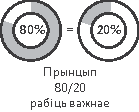
\includegraphics[scale=1.5]{willpower/ch3/10.pdf}
\end{figure}

\textbf{Мы можам выбраць мінімум самых важных дзеяньняў, каб атрымаць большую частку ад заплянаванага поўнага выніку.} Напрыклад, для добрай фізычнай формы нам неабавязкова жыць у~спартыўнай зале і штодзень трэніравацца. Дасьледаваньні паказваюць, што нават пяць хвілінаў інтэнсіўных трэніровак за дзень даюць статыстычна заўважны вынік. У харчаваньні мы працягнем атрымліваць ад яго карысьць, калі ў~нас будзе 80\,\% здаровага рацыёну, а~20\,\% мы пакінем на звычайную ежу. Імкнуцца да 100\,\% можа быць занадта нязручна, патрабаваць ад нас зьмены працоўнага графіка, напрыклад, каб своечасова правільна паесьці. Нам дастаткова выкарыстоўваць адну-дзьве тэхнікі расслабленьня, каб зьнізіць узровень стрэсу на 80\,\%, а~не спрабаваць «намаганьнем волі» дамагчыся абсалютнага спакою. Для таго каб атрымаць пачуцьцё кантролю, неабавязкова імкнуцца поўнасьцю кантраляваць усю сытуацыю. Дастаткова дробязі, адной справы, якую мы актыўна распачнём і возьмем яе пад кантроль. Нават невялікі ўчынак ужо вяртае ўпэўненасьць.

\emph{Мы шмат чулі пра хаду і 10\,000 крокаў, а~вось навукоўцы ўпэўненыя, што і 7500 крокаў забясьпечаць большую частку карысьці. Першыя 20 хвілінаў трэніроўкі прынясуць столькі ж (калі ня больш) карысьці, чым наступныя 40 хвілін.}

\subsection*{Адрозьнівайце важнае і карыснае}

У сьвеце існуюць сотні карысных практыкаў, тысячы прыгожых мясьцінаў і мільёны цікавых людзей. Але нам важна навучыцца адрозьніваць у~багацьці прапановаў карыснае і важнае для нашага здароўя. 

\infobox{Вялікая частка здароўя абумоўленая захаваньнем невялікай колькасьці здаровых звычак, а~большасьць нашых праблемаў са здароўем~--- дзеяньнем невялікай колькасьці шкодных.}

Максімальную карысьць дасьць выбар прыемнай для вас практыкі, якая пры мінімальных выдатках часу дае выйгрыш, што іх нашмат перавышае: паляпшэньне таго месца, дзе вы праводзіце большую частку часу, напрыклад спальні і працоўнага стала; камунікацыя з~тымі людзьмі, хто зараджае вас энэргіяй.

\emph{Сілавыя трэніроўкі хаця б два разы на тыдзень~--- гэта паляпшэньне фізычнага стану, нармалізацыя вагі і абмену рэчываў, павышэньне цягавітасьці і інш. Мэдытацыя 10 хвілінаў у~дзень~--- гэта значнае зьніжэньне стрэсу, павышэньне ўсьвядомленасьці і самакантролю, зьніжэньне трывожнасьці, павелічэньне ўзроўню задаволенасьці і шчасьця.}

Ёсьць мноства карысных справаў, якія патрабуюць выразных выдаткаў, але не прыносяць вялікай карысьці або не пазбаўляюць ад патэнцыйных праблемаў. Гэта ня значыць, што вы павінны імі грэбаваць,~--- рабіце іх, калі гэта прыносіць вам задавальненьне, але памятайце пра эфэктыўнасьць. Для высокай эфэктыўнасьці важна сканцэнтравацца на некалькіх ключавых, не заўсёды відавочных рэчах~--- і надаваць увагу ім.

Вось, напрыклад, гараджанін займаецца ёгай: езьдзіць тройчы на тыдзень на заняткі, выдаткоўвае на зборы і на дарогу каля гадзіны ў~адзін бок. Разам за тыдзень атрымлівае шэсьць пустых гадзінаў, а~часам і траўмы празь няправільнае выкананьня нязвыклых для цела асанаў. Прагулка на сьвежым паветры 30 хвілінаў + расьцяжка 10 хвілінаў і дыхальныя практыкаваньні 5 хвілінаў штодня далі б нашмат больш выразны эфэкт. І істотны выйгрыш у~часе.

Модныя практыкі могуць патрабаваць шмат сілаў і ўвагі, і ўсё гэта будзе амаль бессэнсоўна, калі базавыя рэсурсы здароўя не даведзеныя да ладу.

\subsection*{Пытаньні і заданьні}

1. Нешта моднае, нешта вечнае. Згадайце, якімі «моднымі» аздараўленчымі мэтодыкамі вы займаліся? Ці апраўдалі яны чаканьні?

2. Што з~таго, што вы робіце, прыносіць максімальную аддачу? Якое практыкаваньне самае эфэктыўнае для вас? Што найлепш здымае стрэс?

3. Якія аздараўленчыя мэтодыкі ці практыкаваньні не даюць вам чаканага эфэкту? Ці ёсьць у~іх альтэрнатывы, якія вы яшчэ не спрабавалі?


\section{Прынцып эвалюцыйнага падыходу}

Люблю вывучаць і спрабаваць новыя мэтодыкі аздараўленьня, але не сьпяшаюся ўкараняць іх у~жыцьцё. Не таму, што я кансэрватар з~натуры, а~таму, што мне важна пазьбегнуць утоеных рызыкаў. Таму я прыхільнік эвалюцыйнага падыходу што да здароўя.

У працэсе эвалюцыі мы навучыліся прыстасоўвацца да зьменаў навакольнага асяродзьдзя. Вонкавыя сыгналы запускаюць каскады зьменаў і прыстасаваньняў у~нашым арганізьме, якія павялічваюць нашу адаптыўнасьць і станоўча на нас уплываюць. Гэтыя зьмены сыстэмныя, закранаюць як псыхіку, так і цела, і маюць доўгатэрміновыя наступствы. Лекары старажытнасьці разумелі, што для лячэньня неабходна задзейнічаць сілы арганізма, а~ня проста спадзявацца на лекі. 

\infobox{Антычная формула «medicus curat, natura sanat» у~перакладзе з~латыні значыць «лекар лечыць хваробу, але вылечвае прырода».}

Фізычная актыўнасьць, напрыклад, запускае эвалюцыйныя мэханізмы адаптацыі, павялічваючы нашыя рэсурсы здароўя, паляпшаючы працу мозгу і стрэсаўстойлівасьць, фігуру і якасьць энэргіі. За тысячы гадоў людзі знайшлі многія спосабы паўплываць на свой стан. Розныя цывілізацыі, незалежна адна ад адной, выкарыстоўвалі зьмены ў~харчаваньні, цеплавыя працэдуры, масаж, гартаваньне, галаданьне, мэдытацыю, спорт і да т.~п.

\emph{Прынцып эвалюцыйнага падыходу факусуецца на тым, каб актываваць унутраныя рэсурсы арганізма праз прыродныя сыгналы, а~не прамым умяшаньнем у~малекулярныя шляхі. Напрыклад, ёсьць спробы выкарыстоўваць антыдыябэтычны прэпарат мэтфармін для падаўжэньня жыцьця. Сапраўды, ён стымулюе працэс аўтафагіі (самаачышчэньне клетак), прыгнятаючы актыўнасьць mTOR. Але эвалюцыйна больш бясьпечна і эфэктыўна выкарыстоўваць харчовае ўстрыманьне і фізычную актыўнасьць.}

\begin{figure}[htb!]
  \centering
  
\includegraphics[scale=1.5]{willpower/ch3/11.pdf}
\end{figure}

Нашыя гены~--- гэта датчыкі, сэнсары навакольнага асяродзьдзя. Што мы даём арганізму на ўваходзе, тое і атрымліваем на выхадзе. Сілкуючы арганізм якаснымі прадуктамі, атачаючы добрым кліматам, клапатлівымі сябрамі, практыкуючы прабежкі ды шпацыры на сьвежым паветры~--- атрымліваем на выхадзе выдатнае самаадчуваньне і моцнае здароўе. Калі ж вашае сілкаваньне~--- гэта таксічныя навіны, фастфуд, канапа, сацыяльная ізаляцыя, трывогі і стрэс, то не дзівіцеся зьнясіленьню, вычарпанасьці, хранічным і гострым праявам нездароўя.

\subsection*{Здаровы кансэрватызм}

За апошнюю сотню гадоў зьявіліся й зьніклі многія навамодныя мэтодыкі аздараўленьня. Нейкія зь іх былі проста бескарысныя, іншыя~--- адкрыта небясьпечныя. Але правераныя тысячагодзьдзямі рэкамэндацыі па-ранейшаму цудоўна працуюць і атрымліваюць усё больш навуковых пацьверджаньняў. \textbf{Спорт, харчаваньне, сон, кантроль стрэсу~--- усё гэта вывучалі антычныя аўтары, і на сёньняшні дзень гэта працуе лепш за ўсё.}

Важна даваць свайму целу й мозгу тыя сыгналы, для апрацоўкі якіх яны эвалюцыйна адаптаваныя: 
\begin{itemize}
  \item мы часта недаацэньваем важнасьць сацыяльнага асяродзьдзя, а~людзі вакол нас і дачыненьні зь імі~--- гэта найважнейшы стымул для мозгу;
  \item нам здаецца, што асаблівай розьніцы паміж цьвёрдым яблыкам і сокам або смузі няма~--- але для нашага арганізма розьніца адчувальная;
  \item мы лічым, што зьмена нашага графіка ня мае значэньня, але рэжым дня крытычна важны для здароўя, бо ўзровень гармонаў і актыўнасьць генаў кіруецца цыркаднымі рытмамі, таму парушэньне рэжыму неўзаметку, але моцна ўплывае на самаадчуваньне.
\end{itemize}

Магчыма, неўзабаве мы зможам рэдагаваць свой геном і будзем лягчэй адаптавацца да зьменлівага асяродзьдзя. Але пакуль гэтага няма, давайце паважаць свае гены~--- і яны адкажуць нам узаемнасьцю. Калі мы даём нашаму арганізму тое, што яму трэба, ён адгукнецца з~удзячнасьцю.

Чалавек~--- істота лянівая, імкнецца дасягнуць большага меншымі намаганьнямі. Таму багата хто прагне атрымаць адну таблетку ад усіх хваробаў, хоча знайсьці спосабы стаць прыгажэйшым, разумнейшым і зграбнейшым, не прыкладваючы да гэтага асаблівых намаганьняў. Так, цяпер існуе мноства прэпаратаў, што выбіральна ўплываюць на тыя ці іншыя функцыі арганізма: можна павысіць сваю працаздольнасьць, узьняць настрой, нават крыху схуднець. Але праблема ў~тым, што, узьдзейнічаючы новым спосабам, мы прыкметна павялічваем рызыку ўскладненьняў. 

\infobox{Перавага эвалюцыйнага падыходу ў~тым, што за мільёны гадоў наш арганізм ідэальна прыстасаваўся да ўзьдзеяньня звыклых стымулаў. А стымул у~выглядзе новага прэпарата можа актываваць пабочныя мэтабалічныя або рэгулятарныя шляхі і мець схаваныя доўгатэрміновыя эфэкты.}

\subsection*{Мэдыкамэнтозны падыход vs эвалюцыйны}

Мэдыкамэнтозны падыход ігнаруе прычыны ўзьніклага стану і дзейнічае як абязбольвальнае, прыглушаючы сымптомы і не запавольваючы разьвіцьця стану, якое выклікала праблему. Эвалюцыйны падыход, наадварот, расцэньвае ўзьніклы стан як «неадпаведнасьць» запатрабаваньняў арганізма і рэальнага стану рэчаў. Высьвятляючы такія прычыны, узьдзейнічаючы непасрэдна на лад жыцьця, на рэсурсы здароўя, мы можам заўважна зьмяніць стан чалавека. Эвалюцыйны падыход дзейнічае «па-добраму», улічваючы запатрабаваньні арганізма.

\emph{На жаль, шматлікія людзі выбіраюць дзейнічаць «па-дрэннаму», што дазваляе часова дасягнуць мэты, але з~нанясеньнем шкоды арганізму: схуднець на экстрэмальна нізкакалярыйных дыетах, набраць цягліцы на стэроідных гармонах, падняць настрой вугляводамі, расслабіцца алькаголем і да т.~п. Такія падыходы здольныя разбурыць здароўе вельмі хутка.}

Нам як віду карысьней~--- і прыемней~--- хадзіць нагамі, таму перастаньце карыстацца мыліцамі ў~выглядзе мэдыкамэнтозных спосабаў. Узмацняйце стрэсаўстойлівасьць, а~ня піце транквілізатары, паляпшайце сон, а~не закідвайцеся снатворнымі, выбудоўвайце харчаваньне, а~ня ежце дадаткі.

\subsection*{Палепшыць харчаваньне}

Замест таго каб сфакусавацца на стварэньні рэжыму здаровага харчаваньня, многія аддаюць перавагу ядзе абы-чаго, дадаючы розныя БАДы. Але дасьледаваньні паказваюць, напрыклад, што рыбу немагчыма замяніць рыбіным тлушчам, папулярны дадатак Амэга-3 дзейнічае слаба. Чаму? Рыба~--- гэта ня толькі Амэга-3, але й якасны бялок, мноства мінэралаў, уключаючы цынк, сэлен, ёд ды іншыя, астаксанцын, таўрын і дзясяткі іншых злучэньняў.

Не спрабуйце замяніць гародніну парашком клятчаткі, мяса~--- соевым заменьнікам, а~салату~--- жменяй пігулак. У расьлінах утрымліваюцца сотні фітанутрыентаў, а~ў дадатку ўсяго адзін, пры гэтым у~высокай канцэнтрацыі, таму ён больш таксічны для печані. Магчыма, у~будучыні прыдумаюць цалкам штучную ежу, карысьнейшую за натуральную, але пакуль да гэтага даволі далёка. Будзьма кансэрватыўнымі і аддавайма перавагу сьвежай гародніне з~рыбай дзікае лоўлі.

\emph{Міт пра цукразаменьнікі. Ці можна ашукаць сябе з~карысьцю для арганізма? На жаль, ужываньне цукразаменьнікаў не дапамагае прыкметна схуднець. Праблема цукразаменьнікаў у~тым, што яны эфэктыўна замяняюць цукар: аспартам у~250, а~цукарынат у~520 разоў саладзейшы за цукрозу. Салодкі смак успрымаецца адмысловымі клеткавымі рэцэптарамі салодкіх рэчываў~--- гэта дымэр з~двух рэцэптарных бялкоў T1R2 і T1R3. Калі б яны разьмяшчаліся толькі на языку, праблемаў не было б. Але яны ёсьць і ў~мностве іншых органаў. Усмоктваючыся, цукразаменьнікі інтэнсіўна зьвязваюцца з~рэцэптарамі салодкага смаку ў~падстраўніцы, мозгу, крывяносных сасудах, касьцях, страўніку, кішачніку, тлушчавай тканцы. Так, быццам бы бяскрыўдныя рэчывы істотна зьмяняюць выдзяленьне кішачных гармонаў, парушаюць экспрэсію бялкоў-пераносчыкаў глюкозы, уплываюць на выдзяленьне інсуліну і ўзровень глюкозы ў~крыві~--- пры поўнай адсутнасьці цукру. Акрамя таго, T1R3 ёсьць у~страўніку на грэлін-прадукавальных клетках, і іх залішняя стымуляцыя ўзмацняе апэтыт.}

\infobox{Цукразамяняльнікі могуць павялічваць рызыку дыябэту, уплываць на стан костак, тонус маткі і мачавога пухіра, і нават на стан сасудаў галаўнога мозгу!}

Людзі, якія ўжываюць цукразаменьнікі, часьцей выбіраюць высокакалярыйныя прадукты на працягу дня: у~дасьледаваньні група, якая ўжыла цукразаменьнікі, амаль у~тры разу часьцей выбірала цукеркі, чым тыя, хто піў звычайную або цукровую ваду.

Ужываньне цукразаменьнікаў нэгатыўна ўплывае на дафамінавую сыстэму мозгу і мігдаліну, парушаючы іх працу, пагаршае мазгавы водгук на ўжываньне іншых салодкіх прадуктаў, зьніжаючы адчувальнасьць да салодкага. Цукразаменьнікі ўплываюць на працу прэфрантальнай кары, яны маюць эфэкт прыняцьця рашэньняў у~мадэлі «абясцэньваньня будучыні», калі фокус увагі ссоўваецца толькі на кароткатэрміновыя мэты.

\subsection*{Напампаваць цягліцы}

Многія людзі хочуць мець моцную мускулістую фігуру. Сапраўды, здаровы лад жыцьця, добры сон, правільны рэжым трэніровак, харчаваньне дазваляюць нам падтрымліваць добры ўзровень тэстастэрону і нарошчваць цяглічную масу. У залежнасьці ад генэтыкі, гэты працэс можа ісьці па-рознаму, але прагрэс ёсьць ва ўсіх і абавязкова. Працэс гэты доўгі, мы ж ня толькі нарошчваем цягліцы, але й разьвіваем волю і цярпеньне. Захаваньне такога ладу жыцьця карыснае для здароўя ня толькі дзякуючы росту цягліцаў, але й праз мноства іншых карысных эфэктаў.

Калі хочуць «падмануць прыроду» і «атрымаць фігуру» хутка, часта ўжываюць стэроідныя гармоны: гэта дае прыкметны вынік без усіх умоваў. Чалавек можа нарошчваць цягліцы, не асабліва строга выконваючы рэжым і нават менш трэніруючыся. Але заплаціць за такое неэвалюцыйнае ўмяшаньне давядзецца вялікую цану: зьніжэньне выпрацоўкі ўласнага тэстастэрону, атрафія яечкаў, павелічэньне ўзроўню эстрагенаў, бясплодзьдзе, павелічэньне ціску, паражэньне печані, паскарэньне разьвіцьця атэрасклерозу і рызыка сардэчна-сасудзістых захворваньняў, памяншэньне таўшчыні кары мозгу, павелічэньне рызыкі дэпрэсіі, канцэнтрацыі ўвагі, агрэсіўнасьці і да т.~п. Зразумела, нічога агульнага са здароўем гэта ня мае.

А яшчэ многія «імітуюць» цягліцы, зьвяртаючыся да ін'екцый прэпаратаў, што візуальна іх павялічваюць, або да плястычных апэрацыяў. Напампоўвайце цягліцы, а~ня Эга!

\subsection*{Пытаньні і заданьні}

1. Калі перад вамі стаіць мэта палепшыць нейкі паказьнік, то разглядайце ня толькі мэдыкамэнтозныя мэтады, але й мэтады зьмены ладу жыцьця. Іх камбінацыя часта вельмі эфэктыўная.

2. Як вы прывыклі ўплываць на сваё здароўе: змагацца з~сымптомамі ці высьвятляць прычыну стану?

3. Якія з~новых мэтодыкаў «біяхакінгу» і «ўзлому арганізма», прапанаваныя апошнім часам, былі спалучаныя з~сур'ёзнымі пабочнымі эфэктамі?


\section{Прынцып «бочкі Лібіха»}

Калі ў~труме карабля зьяўляецца вада, то каманда ня проста яе вычэрпвае, а~актыўна шукае прабоіну. Што ж да здароўя, то людзі часта змагаюцца з~наступствамі замест высьвятленьня і ліквідацыі прычыны, прычым марнуюць на гэта шмат часу і сіл. Для таго каб максімальна хутка палепшыць свой стан і падняць узровень энэргіі, трэба знайсьці свае «прабоіны»~--- парушэньні здароўя.

\textbf{Працягваючы марскую тэматыку: караблю небясьпечныя ня ўсе прабоіны, а~толькі тыя, што знаходзяцца ніжэй за ватэрлінію, так і розныя адхіленьні здароўя маюць для нас розную значнасьць.} Уявіце сабе бочку з~рэбрамі рознай вышыні. Колькі вады там можа зьмясьціцца? Правільна, па ўзроўні самага нізкага рабра. Мы можам уявіць сабе, што розныя рэбры~--- гэта рэсурсы здароўя, а~ўзровень вады~--- гэта ваш запас здароўя і энэргіі. З чаго трэба пачаць, каб узьняць узровень здароўя? Зразумела, з~самага слабога зьвяна. Выявіць яго можна, вымераўшы свае рэсурсы здароўя і прааналізаваўшы, якія зьмены мацней за ўсё вам шкодзяць і горш пераносяцца?

\begin{figure*}[htb!]
  \centering
  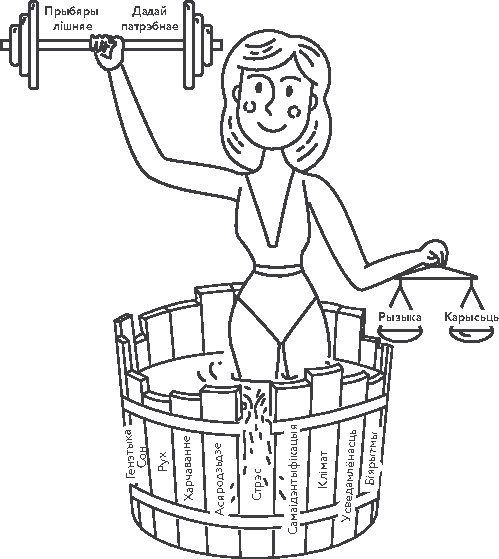
\includegraphics[scale=1.5]{willpower/ch3/12.pdf}
\end{figure*}

\textbf{Пачынаць паляпшэньне здароўя трэба з~выяўленьня свайго самага слабога зьвяна.} Прынцып бочкі Лібіха, ён жа тэорыя абмежаваньня сыстэмы, пастулюе, што трываласьць сыстэмы вызначаецца самым слабым яе кампанэнтам, або, інакш кажучы, арганізму важнейшае за ўсё дзеяньне чыньніка, які найболей адхіляецца ад нормы. Ці працуе гэты прынцып і ўнутры аднаго рэсурсу здароўя?

\emph{Маючы слаба разьвітыя цягліцы корпуса, ня варта павялічваць вагу ў~сілавым спорце, інакш будзе рызыка траўмы. Няма сэнсу старацца ў~выбары салаты, калі вы ня можаце арганізаваць устойлівы рэжым харчаваньня. Не высыпаючыся нармальна, ня варта ўзмоцнена трэніравацца або цярпець голад.}

Нямецкі аграхімік Юстус фон Лібіх устанавіў, што прадуктыўнасьць ураджаю залежыць ад канцэнтрацыі ў~глебе таго мінэралу, узровень якога найменшы: бессэнсоўна ўгнойваць азотам, калі не хапае калію. 

\infobox{Так і ў~здароўі~--- адна з~самых распаўсюджаных памылак людзей у~тым, што яны ня робяць тое, што трэба, і паляпшаюць тое, што ў~іх і так у~парадку.}

У розных людзей, у~залежнасьці ад іх генаў, выхаваньня і г.~д., рэсурсы здароўя могуць мець шырокі дыяпазон талерантнасьці ў~адносінах да аднаго чыньніка і вузкі дыяпазон адносна іншага. Хтосьці больш устойлівы да стрэсу, а~хтосьці моцна пакутуе ад недасыпу. Адзін чалавек добра засвойвае тлушчы, а~іншы дрэнна~--- фруктозу. Калі вы прапампавалі адзін са сваіх рэсурсаў, далейшае яго прапампоўваньне не прывядзе да павелічэньня здароўя.

Так, дасягнуўшы свайго оптымуму рухальнай актыўнасьці, далейшае яе павелічэньне ў~выглядзе звышдоўгіх маратонаў наўрад ці дадасьць здароўя. У гэтым месцы важна зноў прааналізаваць сябе і свой стан, выявіць наступны абмяжоўвальны рэсурс і пачаць надаваць увагу яму. Не здаючы дасягнутых пазыцый, трэба асвойваць усё новыя і новыя, затым вяртацца да ўжо засвоеных, каб палепшыць іх на новым, больш высокім узроўні.

% ((прыбяры лішняе дадай патрэбнае))

\emph{Напрыклад, калі ў~вас начны апноэ, гэта можа блякаваць вашыя намаганьні ў~схудненьні. Калі вы мала рухаецеся, тое дужаньне з~дэпрэсіяй будзе не такое эфэктыўнае.}

Зь іншага боку, павелічэньне нагрузкі можа зрабіць некаторыя чыньнікі неаптымальнымі. Калі вы пачняце шмат займацца, вам спатрэбіцца больш сну для кампэнсацыі. Калі будзеце сутыкацца зь вялікай колькасьцю зьменаў, павысіцца нявызначанасьць, і вам для захаваньня здароўя спатрэбіцца больш высокі ўзровень стрэсаўстойлівасьці.

Разгледзім яшчэ некалькі прынцыпаў, падобных да бочкі Лібіха ў~сваім уплыве на здароўе.

\subsection*{Прынцып атручанай стралы}

У выпадку небясьпечных сытуацыяў важна дзейнічаць неадкладна, а~не разважаць ці аналізаваць. 

\emph{Будыйская прытча пра чалавека, параненага атручанай стралой: сябры спрабуюць выняць стралу, а~ён не дае і засыпае іх пытаньнямі: «Скажыце перш, чыя гэта страла? Хто стрэліў? Зь якога ён горада? Зь якога лука стрэлілі? Колькі праляцела страла? Ня дам выцягнуць стралу, пакуль усё не даведаюся». Так і памёр ад раненьня той чалавек.}

Калі ў~вашым жыцьці ёсьць хваробы ці сытуацыі, якія сур'ёзна пагражаюць вашаму здароўю, перарывайце іх радыкальна. Не чытайце ў~інтэрнэце пра віды стрэл~--- вырвіце стралу! Дзеяньне, а~не разважаньне, першаснае: толькі дзейнічаючы, мы даможамся паляпшэньня свайго стану.

\subsection*{Прынцып «закрыцьця дзірак»}

Гэты прынцып я часта выкарыстоўваю на кансультацыях. Калі мы абмяркоўваем аналізы і лад жыцьця, то ў~першую чаргу плянуем «закрыць дзіркі». Гэта значыць выявіць і ўхіліць наймацнейшыя і небясьпечныя дэфэкты ў~нутрыцэўтычных дэфіцытах, у~крыніцах стрэсу і да т.~п. Чым мацнейшае адхіленьне паказьніка ад нормы, тым большы ўплыў ён аказвае на арганізм і тым важней аднавіць яго балянс.

\subsection*{Прынцып ахілесавай пяты}

Гэты прынцып мяркуе, што важна вывучыць і выявіць свае самыя слабыя месцы і абараніць іх. «Дзе коратка, там і рвецца»: у~выпадках павялічанай нагрузкі мы мацней за ўсё прасядаем у~сваіх слабых месцах, таму важна своечасова іх умацоўваць. Гэта могуць быць і псыхалягічныя трыгеры, і нашыя генэтычныя асаблівасьці, і імунітэт.

\begin{figure}[htb!]
  \centering
  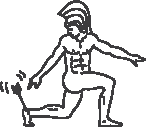
\includegraphics[scale=1.5]{willpower/ch3/13.pdf}
\end{figure}

Падумайце, зь якімі праблемамі са здароўем вы часьцей за ўсё сутыкаецеся і што можна зрабіць, каб перадухіліць іх? Дзе вашае слабое зьвяно? Напрыклад, пры стрэсе ў~адных людзей павышаецца рызыка бессані, у~другіх~--- пераяданьня, у~трэціх~--- павышаецца спажываньне алькаголю. Ведаючы свае слабыя месцы, вы можаце загадзя прыняць захады, каб не дапусьціць зрыву ў~выпадку крытычнай сытуацыі.

\subsection*{Пытаньні і заданьні}

1. Складзіце сьпіс вашых слабых месцаў (фізычных, псыхалягічных, сацыяльных, біяхімічных) і спосабаў іх умацаваньня. Разьмяркуйце іх у~парадку зьніжэньня прыярытэту па ступені ўплыву на вашае здароўе.

2. Што карыснага для сябе вы можаце зрабіць проста цяпер? Папрысядаць? Выпрастацца? Прыняць кантрасны душ? Памэдытаваць 5 хвілінаў?

3. Дзе вы даяце слабіну раней за ўсё пры павелічэньні ўзроўню стрэсу? Як можна перадухіліць гэта?


\section{Прынцып «не нашкодзь»}

\emph{На прыёме ў~лекара пацыент скардзіцца, што ў~яго ўсё баліць. Доктар дабрадушна ўсьміхаецца: «Ну гэта вы загнулі, на ўсё ў~вас ня хопіць грошай».}

Нават калі вы проста пераступаеце парог больніцы, то ўжо рызыкуеце, бо самыя небясьпечныя антыбіётыкаўстойлівыя штамы бактэрыяў часьцей за ўсё «жывуць» менавіта ў~лячэбных установах. Не хачу палохаць вас стацыянарам, але падкрэсьліваю: любое ўмяшаньне можа прынесьці шкоду, а~карысьці «ад лячэньня» пры гэтым выявіцца менш. «Не нашкодзь»~--- так наказваў Гіпакрат, і з~IV стагодзьдзя да н.э. гэты пастулят~--- адзін з~галоўных у~мэдыцыне. 

\infobox{Умець правільна ацэньваць патэнцыйныя рызыкі, патэнцыйную карысьць і іх суадносіны для ўсіх нашых аздараўленчых і лячэбных умяшаньняў вельмі важна.}

Для здаровых людзей рызыка мусіць адсутнічаць або быць мінімальнай~--- гэта тычыцца ўсіх умяшаньняў. Таму не сьпяшаецеся тэставаць на сабе навамодныя мэтодыкі, яны ўжываюцца яшчэ занадта нядоўга, каб можна было выявіць і ацаніць усе магчымыя іх наступствы~--- пабочны эфэкт можа адбіцца празь дзесяцігодзьдзі.

\emph{Як жартуюць лекары, «хворы мае патрэбу ў~доглядзе лекара, і чым найдалей глядзіць лекар, тым лепш»,~--- так таксама бывае часта. І дасьведчаны лекар мусіць умець ня толькі выпісваць, але й адмяняць непатрэбныя лекавыя прэпараты. Нярэдка можна сутыкнуцца, напрыклад, з~пабочным дзеяньнем прэпаратаў у~цяжарных, якое праяўляецца ўжо ў~іх дзяцей. Альбо вось неабгрунтаванае выдаленьне мігдалінаў у~дзяцей, якое ў~тры разы падвышае магчымасьць разьвіцьця хваробаў лёгкіх, а~таксама рызыку рэсьпіраторных, інфэкцыйных і алергічных захворваньняў.}

\textbf{Лячэньне ніколі не павінна быць больш небясьпечным, чым захворваньні!} Для людзей хворых рызыка ад выкарыстаньня пэўнага прэпарата ці з~прычыны апэрацыі апраўданая: чым мацнейшае захворваньне, тым большая рызыка лячэньня дапушчальная. Чым цяжэйшае захворваньне, тым большая карысьць будзе ад апэрацыі або прэпарата~--- суадносіны рызыка / карысьць мяняецца. Таму, напрыклад, антыдэпрэсанты куды больш эфэктыўныя пры цяжкіх дэпрэсіях, чым пры лёгкіх.

\textbf{Правільная ацэнка рызыкі} важная для выбару тактыкі лячэньня. Напрыклад, чым вышэйшая ў~вас рызыка сардэчна-сасудзістых захворваньняў, тым больш агрэсіўнай павінна быць тактыка зьніжэньня «дрэннага халестэрыну» да меншых лічбаў. У складаных сытуацыях зацягваньне праблемы можа адно пагаршаць яе, таму дзейнічаць трэба рашуча. Чым вышэйшая рызыка сьмерці, тым на большыя рызыкі ў~лячэньні можна ісьці. Возьмем праблему хранічнага болю. Кожны выпадак патрабуе дыягностыкі, у~ім трэба разьбірацца і індывідуальна падыходзіць да рашэньня. Але ва ўладзе фармкампаніяў укараніць у~шырокую практыку небясьпечныя прэпараты, прымяншаючы іх пабочныя эфэкты. Ды й лекарам бывае прасьцей прызначыць абязбольвальнае, чым разьбірацца з~прычынай боляў.

\emph{Так у~90-я гады мінулага стагодзьдзі пачалася апіоідная катастрофа ў~ЗША: памятаеце прагу доктара Хаўса да вікадыну? Кінематаграфічны прыклад таго, як бескантрольнае прызначэньне апіоідных анальгетыкаў прывяло да фармаваньня цяжкай залежнасьці, пераходу на наркотыкі ды імклівага росту колькасьці выпадкаў сьмерці ад перадазіровак. Пры немагчымасьці легальна купіць прэпараты, людзі пачалі зьвяртацца ў~крымінальныя структуры, і гэта павялічыла продажы вулічных наркотыкаў. Паводле дасьледаваньняў, да 80\,\% амэрыканцаў, якія выкарыстоўваюць гераін, перайшлі на яго з~абязбольвальных апіоідаў.}

\textbf{«Вельмі часта найлепшы лек~--- гэта абысьціся без яго»}~--- і гэтую мудрую фразу прыпісваюць старажытнагрэцкаму лекару Гіпакрату. Як ведаюць хірургі, найлепшая апэрацыя~--- гэта тая, якую не зрабілі. Калі можна абысьціся без апэрацыі, трэба абысьціся безь яе. Спытайце ў~свайго лекара: а~ці можна яе адкласьці, ці здарыцца што-небудзь страшнае, калі не зрабіць апэрацыю?

\emph{Ёсьць дзясяткі неэфэктыўных апэрацыяў (без даведзенай карысьці), якія робяць па ўсім сьвеце,~--- гэта і некаторыя апэрацыі на сэрцы, і артраскапія каленнага сустава пры артрыце, і шэраг апэрацый на хрыбце, напрыклад унутрыдыскавая электратэрмальная тэрапія. Паляпшэньні пасьля іх часьцей за ўсё зьвязаныя з~плацэба-эфэктам, бо нават пры «фіктыўнай апэрацыі», калі праводзіцца толькі наркоз і надрэз~--- і больш нічога,~--- фіксуецца наступнае заўважнае паляпшэньне самаадчуваньня. Але пры гэтым рызыка ўнутрышпітальнай інфэкцыі, трамбозу і да т.~п. для пацыентаў, якія знаходзяцца ў~стацыянары, вышэйшая ў~разы.}

\emph{Некаторыя віды дыягностыкі пры бяздумным выкарыстаньні таксама могуць нашкодзіць. Напрыклад, каланаскапія нясе рызыкі пашкоджаньня сьценкі кішачніка, таму калі рабіць яе часта людзям да 50 гадоў (а тады выявіць захворваньне малаімаверна), то рызыкі ад дыягностыкі будуць вышэйшыя, чым карысьць. Зрэшты, можна замяніць гэта віртуальнай каланаскапіяй.}

А як можна ацаніць псыхічную шкоду, нанесеную неабгрунтаванымі высновамі і дыягназамі, выпадкова выяўленымі дыягнастычнымі артэфактамі? «Выконваць псыхічную гігіену» лічыў важным псыхіятар Уладзімір Бехцераў, і ўжо больш за сто гадоў гэтая ідэя застаецца актуальнай. Гісторыя поўніцца выпадкамі ятрагеніяў, то бок пагаршэньняў фізычнага ці эмацыйнага стану чалавека, ненаўмысна справакаваных мэдыцынскім працаўніком. Цікава, што зь сёньняшніх мэтадаў і падыходаў будзе прызнана небясьпечным і шкодным у~найбліжэйшай будучыні? 

\infobox{Пакуль варта памятаць, што ўстрымлівацца ад непатрэбных абсьледаваньняў і прэпаратаў для ўмоўна здаровых людзей ня менш карысна для здароўя, чым своечасова рабіць патрэбныя абсьледаваньні.}

\subsection*{Чаму ўзьнікае залішняе ўмяшаньне?}

Калі да лекара прыходзіць пацыент і ў~яго ёсьць скаргі, то псыхалягічна складана адпусьціць яго з~агульнымі рэкамэндацыямі. Ды і пацыенты хочуць прызначэньняў~--- патураньне гэтым запытам прыводзіць да прызначэньня непатрэбных абсьледаваньняў і прэпаратаў. Цяжка ўстрымацца ад таго, каб нічога не прызначыць. 

\emph{Як жартуюць, цяпер існуе так шмат розных прэпаратаў, што даводзіцца прыдумляць новыя хваробы, каб іх прызначаць.}

Таксама мы можам недаацэньваць шкоду умяшаньняў і мэтодыкаў праз кагнітыўнае скажэньне, калі адмоўныя вынікі і пабочныя эфэкты замоўчваюцца. Гэта адбываецца як адмыслова, калі ў~выпрабаваньнях заніжаюцца пабочныя эфэкты прэпаратаў, а~спэцыялізаваныя часопісы не публікуюць артыкулы аб прэпаратах, якія не паказалі эфэктыўнасьці, так і не адмыслова, калі тыя, каму не дапамагло, замоўчваюць пра гэта, а~тыя, каму стала лягчэй, шырока дзеляцца сваімі ўражаньнямі. Такая асымэтрыя вядзе да няслушнай адзнакі рызык.

\subsection*{Вывучайце рызыкі}

Рызыка~--- гэта не сярэдняе значэньне, а~індывідуальнае. Напрыклад, для адзнакі пабочных эфэктаў лекавага прэпарата важна ўлічваць узрост пацыента, існыя захворваньні, зьвесткі абсьледаваньняў і лябараторныя паказьнікі. Даведайцеся ўсе фактары рызыкі і пэрсаналізуйце іх. Таксама важна пэрсаналізаваць і пасьпяховасьць лячэньня. Цяпер можна загадзя, на падставе генэтычнага тэсту, ацаніць імавернасьць пасьпяховага лячэньня шэрагу захворваньняў, напрыклад гепатыту С або дэпрэсіі, пэўнымі прэпаратамі, выбраўшы найбольш эфэктыўны менавіта для вашага геному.

Калі мы гаворым пра зьмяненьне ладу жыцьця, то спорт і дыеты не такія бясьпечныя, як можа падацца на першы погляд. Таму важна ацэньваць і іх рызыкі, вывучаць чужыя няўдачы~--- часта яны могуць несьці больш карыснай інфармацыі, чым посьпехі. Мы можам прыняць меры і зьнізіць свае рызыкі загадзя, асабліва калі ведаем тыповыя пагрозы і памылкі. На жаль, людзі, у~якіх нешта не атрымалася, нячаста дзеляцца нэгатыўным досьведам.

\subsection*{ЗЛЖ кухоннай кнігі}

Людзі любяць хуткае вырашэньне ўсіх праблемаў са здароўем праз прыём дабавак і лекаў і ўвесь час знаходзяцца ў~пошуку «адной пігулкі ад усіх хваробаў». Як рыцары караля Артура шукалі чару Грааля, якая вылечвае ад хваробаў і дае неўміручасьць, так і сёньня людзі шукаюць у~сацсетках схэмы прыёму дадаткаў. Рашэньне практычна любой праблемы са здароўем можна зьвесьці да прыёму набору БАДаў. Проста як у~магічным рэцэпце: як узыдзе поўня, вазьмі тоўчаныя мышыныя языкі, сэрца шыбеніка і корань мандрагоры; а~цяпер гучыць: замоў дадатак 1, дадатак 2 і дадатак 3. \textbf{Пэрыядычна ў~шматлікіх людзей пачынаецца сапраўдны сьверб, маўляў, чаго б такога мне прапіць?}

Абсалютная большасьць гэтых злучэньняў у~лепшым выпадку бескарысныя, а~іх прыём можа адцягваць чалавека ад сапраўды важных мерапрыемстваў. Лепш бы выдаткаваць гэтыя сілы на паляпшэньне харчаваньня або спорт. Бо зьвесткі пра карысьцт гэтых дабавак могуць быць атрыманыя на клеткавых культурах, на жывёлах і не пераносяцца на чалавека. Нават калі вы спрабуеце зьмяніць дадаткамі нейкі біяхімічны паказьнік, яго зьмена не заўсёды будзе гаварыць аб карысьці для здароўя. Таму навукоўцы дасьледуюць уплыў прэпаратаў ня толькі на «мяккія пункты» (г.~зн. прамежкавыя паказьнікі), але заўсёды~--- на «цьвёрдыя пункты» (працягласьць жыцьця і частасьць ускладненьняў). Напрыклад, зьніжэньне цынку пры дэпрэсіі адбываецца не празь яго дэфіцыту, а~празь пераразьмеркаваньне. Павышэньне гомацыстэіну можа быць і праз парушэньне работы нырак, а~не дэфіцыт вітамінаў B\textsubscript{9} і B\textsubscript{12}.

Многія нават лекавыя прэпараты, якія паляпшаюць стан пацыентаў, у~выніку могуць павялічваць іх сьмяротнасьць: напрыклад, шэраг лекаў пры мігальнай арытміі. Бывае і так, што прэпараты, якія спачатку нават крыху пагаршаюць стан пацыентаў, напрыклад бэта-блякатары, у~выніку падаўжаюць ім жыцьцё. Таму так важна прытрымлівацца доказнай мэдыцыны замест таго, каб верыць сваім суб'ектыўным адчуваньням або чаканьням.

У залежнасьці ад чалавека, праблемай можа быць і дэфіцыт, і лішак якога-небудзь рэчыва, праілюструю на прыкладзе жалеза. Калі жалеза ў~арганізьме бракуе і ўзровень фэрытыну (паказвае запасы жалеза) нізкі, гэта можа быць прыкметай жалезадэфіцытнай анэміі, якая моцна пагаршае самаадчуваньне і часта сустракаецца ў~жанчынаў. У гэтым выпадку прэпараты жалеза дапамогуць.

А вось мужчыны часьцей сутыкаюцца з~павышаным фэрытынам. Лішак жалеза павялічвае рызыку шматлікіх захворваньняў, у~гэтым выпадку паказана донарства, а~калі ён пачне проста піць дадаткі жалеза, гэта пагоршыць яго стан. Проста піць такія дадаткі без высьвятленьня прычынаў няварта, бо хранічная анэмія ў~пажылых можа быць і праз крывацёкі, абумоўленыя ракам кішачніка, а~можа быць і праз інфэкцыю.

\subsection*{Пытаньні і заданьні}

1. Ці разьлічваеце вы рызыкі (як бліжэйшыя, так і аддаленыя) і перавагі пры выкарыстаньні лекавых прэпаратаў або плянаваньні апэрацыяў?

2. Ці прытрымліваецеся вы ці ваш лекар прынцыпу «не нашкодзь»?

3. Займаючыся аздараўленьнем, ці ўяўляеце вы рызыкі працэдур або тэхнік і спосабы іх мінімізацыі?


\section{Прынцып штангі}

Прынцып штангі~--- гэта спалучэньне некалькіх падыходаў у~адным рэсурсе здароўя, калі для вырашэньня адной праблемы даюцца дзьве парады: пазітыўная~--- што рабіць, і нэгатыўная~--- чаго не рабіць. Напрыклад, у~харчаваньні важна як пазьбягаць цукру, так і дадаваць больш гародніны. Для фізычнай актыўнасьці~--- пазьбягаць гіпадынаміі нават важней, чым рэгулярна трэніравацца. Для якасьці сну важна як пазьбягаць сьвятлодыёднага сьвятла ўвечары, так і бываць днём на вуліцы. \emph{(Навошта~--- спытаеце вы? А таму, што ультрафіялетавы спэктар удзельнічае ў~выпрацоўцы сератаніну, а~сератанін зьяўляецца папярэднікам начнога гармону мэлятаніну, падрабязьней пра гэта~--- у~разьдзеле «Сон»).}

Прынцып штангі таксама мяркуее выкарыстаньне дзьвюх самых эфэктыўных стратэгій, ігнаруючы прамежкавыя, менш важныя. \textbf{Гэта значыць~--- рабіць самае карыснае для сябе і ўстараняць самае небясьпечнае.} Устараненьне самага небясьпечнага мае на ўвазе мінімізацыю рызыкаў, раньнюю дыягностыку~--- гэта дапамагае пазьбегнуць або выявіць на раньняй стадыі захворваньні, якія пагражаюць жыцьцю. Напрыклад, чым раней распачатае лячэньне сардэчна-сасудзістых або ракавых захворваньняў, тым вышэйшая імавернасьць спрыяльнага зыходу.

Устараненьне пагрозаў~--- гэта і такія прафіляктычныя мерапрыемствы, як вакцынацыя. Пра стандартныя пляны вакцынацыі напісана ўжо шмат, адзначу толькі, што прышчэпкі ратуюць ня толькі ад інфэкцыйных захворваньняў, але ад ракаў, напрыклад прышчэпка ад папілёмавірусаў (цэрварыкс, гардасіл). Яна ратуе ня толькі ад раку шыйкі маткі, але і ад плоскаклетачных ракаў (у першую чаргу ротаглыткі). З узростам імунітэт аслабляецца і некаторыя прышчэпкі трэба паўтарыць. А вось пажылым людзям таксама важна зрабіць дадатковыя прышчэпкі супраць узбуджальнікаў пнэўманіі, напрыклад вакцыну супраць пнэўмакоку (прэвэнар).

\subsection*{Лячыць хваробы ці ўмацоўваць здароўе?}

Часта і дактары, і пацыенты блытаюць гэтыя рэчы. Зьвяртаючыся да лекара, людзі часам чуюць: «Вы здаровыя, хваробы няма». У такіх выпадках паляпшэньне самаадчуваньня будзе прыходзіць пры ўмацаваньні здароўя. Але калі ёсьць канкрэтнае захворваньне, то трэба, вядома, сфакусавацца на яго лячэньні. Напрыклад, прымаць супрацьвірусныя прэпараты пры віруснай інфэкцыі, антыбіётыкі~--- пры бактэрыяльнай інфэкцыі, рабіць апэндэктамію пры апэндыцыце і да т.~п. Зрэшты, як я пісаў у~папярэднім разьдзеле, цяпер усё большае распаўсюджваньне атрымліваюць «хваробы цывілізацыі», такія як атлусьценьне, цукровы дыябэт 2 тыпу, дэпрэсія, алергіі і аўтаімунныя захворваньні. 

\textbf{Прычына гэтых захворваньняў~--- лад жыцьця, таму прыдумаць адну таблетку, якая вылечыць іх, амаль немагчыма.} Мэдыцына прапануе «кантраляваць» іх сымптомы на працягу ўсяго жыцьця, бяз спробы вылечыцца цалкам. Але ў~такім выпадку зьмена ладу жыцьця эфэктыўнейшая за любыя прэпараты: так, цукровы дыябэт 2 тыпу ў~многіх выпадках можна вылечыць. Так, гэта складана, але гэта будзе сапраўднае лячэньне, а~не «кантроль сымптомаў».

\subsection*{Прынцып нэгатыўных парадаў} 

Калі ў~знакамітага скульптара Мікеланджэла спыталі, як яму ўдаецца ствараць такія цудоўныя статуі, ён адказаў: «Я бяру глыбу мармуру і адсякаю ад яе ўсё лішняе». 

\infobox{Вы можаце ўчыніць са сваім ладам жыцьця, як Мікеланджэла са сваімі статуямі,~--- прыбраць усё лішняе. А потым ужо можна дадаваць нешта, не перагружаючы сябе.}

Усе рэкамэндацыі адносна здароўя можна ўмоўна падзяліць на пазітыўныя парады «рабі гэта» і нэгатыўныя «не рабі гэтага». Цікава, што парады «не рабі» звычайна маюць больш высокую навуковую дакладнасьць і, як правіла, асабліва не зьмяняюцца зь цягам часу. А вось пазітыўныя парады часта выяўляюцца няпэўнымі, недакладнымі. Пазітыўныя парады патрабуюць больш часу на выкананьне, пакідаюць меней гнуткасьці і магчымасьці выбару. Таму й на кансультацыі я таксама аддаю перавагу распачаць з~таго, што можна перастаць рабіць дзеля лепшага здароўя.

\emph{Напрыклад, у~дыеталёгіі розныя спэцыялісты бадай ня маюць разыходжаньняў у~поглядах на тое, якая ежа шкодная для здароўя: фастфуд, смажаная, рафінаваныя вугляводы, цукар і да т.~п. Пры гэтым ёсьць прыкметныя адрозьненьні ў~тым, што карысьнейшае~--- ці то тлушчы, ці то расьлінная ежа. Усе згодныя, што гіпадынамія шкодная, але вядуцца спрэчкі аб тым, які від спорту карысьнейшы.}

Ёсьць шмат модных спосабаў паляпшэньня здароўя, накшталт стрэтчынгу, інфрачырвоных лямпаў, стымуляцыі мозгу, але падумайце лепш, што можна перастаць рабіць, і складзіце свой сьпіс.

\textbf{«Не рабіць» добрае тым, што вызваляе вашыя сілы і час і дапамагае сканцэнтраваць увагу.}

У сьпіс «не рабіць» могуць увайсьці чыньінкі, якія зьнясільваюць вас. Якія шкодныя ўзьдзеяньні можна ўхіліць, няхай гэта будзе паветра, вада, шум, сьвятло? Як можна датрымлівацца эмацыйнай гігіены, каб паменшыць нэгатыўнае ўзьдзеяньне навязьлівых думак, крыўдаў, чаканьняў, жаданьняў? Што можна выкінуць з~дому, каб стаць больш здаровымі? Напрыклад, стары дыван, які назапашвае велізарную колькасьць пылу.

«Калі гэта не адназначнае так, то гэта адназначнае не». Што да працы і вашага здароўя, правіла «не рабі» дакладнейшае і карысьнейшае, чым правіла «рабі». Мы ведаем пра тое, што няслушна і шкодна, нашмат больш, чым пра тое, што слушна і карысна. Тое, што было ўчора і сёньня няслушным і шкодным, малаверагодна стане слушным і карысным заўтра. А вось наконт карыснага сёньня~--- ня факт! Пакідайце лішняе, вызваляйце працоўную памяць, матывацыю і запал да новых справаў і ўчынкаў. Не дадавайце лішняга. Вам можа быць шкада вашых старых шкодных звычак, дзейнічайце бязьлітасна і рашуча, як яшчарка, якая адкідае хвост. Вырашайце праблемы замест іх абмеркаваньня і пакідайце іх у~мінулым. Адсякайце лішняе, дзейнічайце рашуча ў~вырашэньні сваіх праблемаў здароўя. Няхай вашай прымаўкай стане хірургічная «Ubi pus, ibi incisio»~--- дзе гной, там разрэз! Ня думайце аб тым, як упускаць у~сваё жыцьцё сотню справаў, думайце, як адмаўляцца і рашуча гаварыць «не» новаму і бліскучаму. Толькі так вы зможаце дасягнуць фокусу і ўвагі. Менш~--- гэта больш. Менш~--- гэта здаравей.

\subsection*{Пытаньні і заданьні}

1. Што можна выкінуць з~галавы, каб стала лягчэй? Які цяжар чаканьняў і крыўдаў вы штодня носіце з~сабой?

2. Што можна зьмяніць у~доме ці асяродзьдзі, каб атрымаць паляпшэньне для здароўя? Што выкінуць, што перастаць чытаць, з~кім з~таксічных людзей перастаць дачыняцца?

3. Што можна перастаць рабіць, каб атрымаць плюсы для здароўя? Складзіце сьпіс.


\section{Прынцып сыстэмы}

Калі людзі гавораць пра здаровыя звычкі, то часта ставяць сабе мэты: напрыклад, прапампаваць грудныя цягліцы, наладзіць сон, схуднець на 5 кг. Але калі мэта дасягнутая, тут жа прыходзіць расслабленьне: людзі кідаюць рабіць тое, што ім дапамагала, і страчваюць усё дасягнутае.

\infobox{Прынцып сыстэмы~--- гэта стварэньне набору звычак, якія ўтрымліваюцца на працягу доўгага часу.}

Не «схуднець на 5 кг», а~«стварыць сыстэму харчаваньня, якая падтрымлівае маю здаровую вагу». Гэты прынцып заклікае выбіраць бясьпечныя для здароўя спосабы, якіх вы зможаце датрымлівацца на працягу многіх гадоў. Сапраўдны клопат пра сябе~--- гэта не галаданьні і зьнясільвальныя трэніроўкі, а~доўгатэрміновы сыстэмны падыход.

Стварыўшы сыстэму, мы пераходзім ад этапу сьвядомых намаганьняў да аўтаматычнай работы звычак. Звычкі і асяродзьдзе ўзьдзейнічаюць на вас кожны дзень, і гэта нашмат мацней, чым валявыя самапрымусы. Больш за тое, эпізадычныя наскокі шкодныя для здароўя. Напрыклад, чым часьцей здараюцца эпізоды ваганьняў вагі больш чым на 5 кг, тым вышэйшая рызыка атлусьценьня. Калі за нас працуе сыстэма, зьмены становяцца надзейней і вагавіцей.

\emph{Памятаеце міф пра аўгіевы стайні? Калі Гераклу загадалі ачысьціць іх, ён узяў рыдлёўку і пачаў капаць. Але чым глыбей ён капаў, тым больш гною сыпалася яму на галаву. Так і мы, намаганьнем разграбаючы свае праблемы, можам яшчэ мацней у~іх закопвацца. Затым Геракл вырашыў выкарыстаць іншы падыход~--- ён перакрыў раку, і яна вымыла ўвесь гной са стайняў. Так і сыстэматычнае зьмяненьне ладу жыцьця дапаможа нам ня проста дасягнуць мэтаў, але й падтрымліваць іх у~доўгатэрміновай пэрспэктыве.}

Для таго каб эфэктыўна кіраваць рэсурсамі здароўя, важна ствараць вакол сябе дабратворнае асяродзьдзе (гэта і людзі, і рэчы, і мейсцы), якое падтрымлівае вас у~дасягненьні мэтаў. Ідэальным стане такое ўкараненьне рэсурсу ў~лад жыцьця, каб ён у~выніку не патрабаваў асобнай практыкі.

\emph{Напрыклад, прынцып ускоснага ўплыву мяркуе непрамое фізыялягічнае ўзьдзеяньне праз трыгеры: поўная цемра, а~не снатворнае, яркае сьвятло, а~не кафэін.}

Па меры таго, як мы асвойваем новыя звычкі, можам пераводзіць іх з~галіны фармальнай практыкі ў~нефармальную: адначасова гуляць на сьвежым паветры, практыкаваць усьвядомленую хадзьбу-мэдытацыю, атрымліваць карысьць і задавальненьне ад сонца~--- гэта яно. Або, да прыкладу гуляць у~тэніс зь сябрам, весьці ў~працэсе перамовы, атрымліваючы задавальненьне і ад гульні, і ад камунікацыі, і ад прыгожага мейсца, у~якім разьмешчаны корт. Гэта вельмі пра здароўе.

\textbf{Стварайце сыстэму звычак,} якія вам падабаюцца і якія вы можаце ўкараніць у~доўгатэрміновай пэрспэктыве, адпрацоўвайце яе да аўтаматызму. Гэта як каляіна, якая будзе падтрымліваць вас і не даваць збочыць са шляху здароўя, нягледзячы на магчымыя перашкоды і цяжкасьці. Для дзяцей важна ствараць такую сыстэму звычак з~самага дзяцінства. Людзі і навукоўцы бясконца спрачаюцца аб тым, які прадукт карысны або шкодны, аб тым, што важнейшае~--- харчаваньне або спорт. Але здароўе~--- гэта сыстэма, а~не адзін прадукт. Таму і здаровае харчаваньне~--- гэта сыстэма, якая ўключае ў~сябе рэжым харчаваньня, выбар прадуктаў, каляраж, харчовую псыхалёгію, гатаваньне і многае іншае. Здароўе аптымальна працуе, толькі калі ўсе элемэнты ягонае сыстэмы задзейнічаныя.

\emph{Узімку вы ня зможаце жыць у~хаце, дзе няма або вокнаў, або дзьвярэй, або падлогі, або даху~--- для таго, каб сагрэцца, неабходныя ўсе яе часткі. Так і са здароўем~--- важна гарманічнае разьвіцьцё ўсіх рэсурсаў здароўя. Успомніце, як сьмешна выглядае чалавек, які напампаваў сабе адно біцэпсы і ходзіць з~«курынымі» лыткамі.}

Сыстэма і прапорцыя~--- вось вашыя правілы. Кожная звычка, пра якую пойдзе гаворка,~--- гэта цагліна ў~трывалай сьцяне вашага здароўя.

\subsection*{Прынцып здаровых звычак}

Цяпер пры ацэнцы дзеяньня многіх прэпаратаў, дадаткаў, стратэгій выкарыстоўваюцца канчатковыя пункты ў~выглядзе іх мэтавай эфэктыўнасьці, таксічнасьці, уплыву на пэўныя маркеры. Досыць часта гэтыя дасьледаваньні праводзяцца ў~кароткатэрміновыя прамежкі і могуць ігнараваць доўгатэрміновыя наступствы. Адным з~такіх наступстваў зьяўляецца зьмена паводзінаў. Эканамічныя навукі і біямэдыцынскія дасьледнікі апошнім часам пачалі зьвяртаць больш увагі на тое, як зьмяняюцца нашыя паводзіны, як зьмяняецца наш выбар і перавага рызыкаў. Бо наш выбар~--- гэта нашмат глыбейшая тэма, чым простыя веды аб тым, што карысна, а~што шкодна.

Многія «экспэрты» ігнаруюць паводзінныя патэрны, даючы парады накшталт: «Дэпрэсія? Больш усьміхайся!», «Схуднець? Проста перастань есьці!», «Не атрымліваецца? Старайся мацней». Лягічна? Лягічна! Але такая спрошчаная лёгіка ня будзе працаваць у~складаных сыстэмах, бо сьвядомыя разважаньні і разуменьне сваёй праблемы далёка не заўсёды прыводзяць да зьмены паводзінаў.

\emph{Гучыць як насьмешка, але да гэтага часу можна пачуць: «Атлусьценьне? Проста лічы калёрыі!» Аднак харчовыя паводзіны~--- гэта складаны нэўраэндакрыны працэс, які зьвязвае разам узровень фізычнай актыўнасьці, ежу, стрэс, сьвятло й дзясяткі іншых чыньнікаў. На працягу дня чалавек неўзаметку для сябе прымае больш за 500 харчовых рашэньняў~--- і калі праходзіць міма кавярні з~водарам выпечкі, і калі адкрывае дома лядоўню. Немагчыма «кіраваць» усімі гэтымі аспэктамі паводзінаў.}

\infobox{Чалавек, які цешыцца хуткаму пахуданьню на цвёрдай абмежавальнай дыеце, падобен на рабаўніка, які купаецца ў грашах, калі па ўсходах ужо падымаецца паліцыя, каб яго арыштаваць.}

Харчовыя паводзіны павінны быць заснаваныя на звычках, якія мы самі можам лёгка кантраляваць. Напрыклад, лічыць гадзіны пры рэжыме харчаваньня або інтэрвальным галаданьні, замест таго каб лічыць калёрыі, якія мы ня можам ацаніць дакладна. Сьвядомы харчовы кантроль у~стрэсавым асяродзьдзі немагчымы на доўгатэрміновай падставе, таму эфэктыўнасьць абмежавальных дыет засмучальна малая~--- каля 5\,\% посьпеху ў~доўгатэрміновай пэрспэктыве. Чалавек, які радуецца хуткаму пахудзеньню на жорсткай абмежавальнай дыеце, падобны да рабаўніка, які купаецца ў~грашах, калі па лесьвіцы ўжо паднімаецца паліцыя, каб яго арыштаваць.

Харчовыя паводзіны~--- гэта набор звычак, аўтаматычных рэакцый, якія парадкуюць наша харчаваньне ў~доўгатэрміновай пэрспэктыве. Так, вы можаце зьесьці колькі хочаце, але, выбіраючы ежу нізкай спэцыфічнай калярыйнасьці і сілкуючыся два разы на дзень, даволі складана атрымаць залішнюю вагу, нават калі вельмі імкнуцца. Але самае галоўнае ў~гэтай справе~--- шматгадовы ўстойлівы трэнд здаровай вагі, падтрымаць які могуць толькі звычкі, а~не вясновыя наскокі на абмежавальныя дыеты. Усе нашыя даволі бедныя рэсурсы ўсьвядомленасьці варта вытрачаць не на падлік калёрыяў, а~на выпрацоўку новых звычак. 

\emph{50\,\% здароўя~--- гэта здаровыя звычкі.}

\subsection*{Пытаньні і заданьні}

1. Як вы можаце ўкараніць здаровыя звычкі ў~свой рэжым жыцьця, працу і адпачынак? Як вы можаце спалучаць адразу некалькі здаровых звычак?

2. Ці было так, што дасягненьне мэты ў~здароўі прыводзіла вас да страты матывацыі і адмовы ад далейшых дзеяньняў?

3. Ці патрапляеце вы дабівацца аўтаматызму, выпрацоўкі здаровых звычак на пастаяннай падставе?


\section{Прынцып «выкарыстоўвай або страціш»}

Здароўе цяжка назапасіць і ўтрымаць без штодзённага выкарыстаньня. Наш арганізм схільны эканоміць рэсурсы, і калі мы іх не выкарыстоўваем, то яны могуць скарачацца. Таму здароўе~--- гэта здаровы лад жыцьця, тое, што мы робім рэгулярна, а~ў ідэале~--- штодня.

\textbf{Адсутнасьць належных выклікаў у~жыцьці, гострых стрэсаў дэтрэніруе нашу псыхіку і цела.} Напрыклад, калі мы перастаём займацца спортам, то ўжо праз два месяцы ўзровень сілы зьніжаецца, а~праз паўгода вяртаецца да зыходнага стану. Чым даўжэй вы трэніруецеся, тым больш павольна гэта адбываецца. Усяго за 14 дзён адмовы ад трэніровак вы можаце страціць да 12\,\% цяглічнай масы. Калі цалкам спыняюць займацца прафэсійныя спартоўцы, за 2 месяцы трывушчасьць падае на 21\,\%, а~за тры~--- на 50\,\%.

З аднаго боку, рэгулярныя трэніроўкі важныя для захаваньня актыўнасьці і мозгу, і цела, з~другога~--- пастаянная раўнамерная нагрузка не працуе, бо мы хутка да яе адаптуемся. Манатоннасьць і звычнасьць аслабляюць нас, таму заўсёды патрэбныя новыя задачы, новыя сытуацыі. Адаптуючыся да незвычайных умоваў, мы трапляем у~пункты супэркампэнсацыі~--- калі пасьля адаптацыі мы становімся мацнейшымі, чым былі да.

\begin{figure}[htb!]
  \centering
  
\includegraphics[scale=1.5]{willpower/ch3/14.pdf}
\end{figure}

\textbf{Прынцып «выкарыстоўвай або страціш» працуе ня толькі датычна здароўя:} важна выкарыстоўваць свой час, інакш ён выцякае скрозь пальцы. Важна працаваць над адносінамі: пушчаныя на самацёк, яны наўрад ці будуць спантанна паляпшацца. Кожны наш навык закадаваны ў~мозгу ў~нэўронавых сувязях. Гэтыя сувязі плястычныя. Чым часьцей мы актывуем іх, тым больш яны ўмацоўваюцца. Чым радзей, тым вышэйшая рызыка таго, што навык стане слабейшым і можа нават зьнікнуць.

\textbf{Калі мы мала рухаемся, то ня толькі страчваем цяглічную масу, таксама ў~нас у~мозгу памяншаецца колькасьць нэрвовых клетак, якія кіруюць цягліцамі. Таму многія нэўрадэгенэратыўныя захворваньні хутчэй прагрэсуюць пры маларухомым жыцьці.}

Рэсурсы здароўя не пасіўныя, іх немагчыма назапасіць і закансэрваваць, іх трэба рэгулярна выкарыстоўваць. Калі мы сустракаемся з~новымі выклікамі, сутыкаемся са стрэсамі, калі ад нас патрабуецца праявіць волю і сілу, то менавіта колькасьць рэсурсаў вызначае вынік. Чым больш запасу, тым лягчэй мы адаптуемся. Калі ж спрабаваць пазьбягаць складаных задач, не выкарыстоўваць свае патэнцыйныя магчымасьці, то яны пачынаюць памяншацца, адміраць, падпарадкоўваючыся ўжо іншаму прынцыпу~--- скарачэньне непрацуючых функцый, згортваньне функцый празь незапатрабаванасьць.

\subsection*{Прынцып штодзённасьці}

Многія здаровыя звычкі паказваюць сваю максімальную карысьць толькі пры штодзённым, а~не эпізадычным ужываньні. Сон, ежа і трэніроўкі ня могуць быць назапашаныя. За рэдкім выключэньнем, ідэя прыняць шмат вітамінаў за адзін раз і на паўгода~--- шкодная. Многія спрабуюць абысьці гэты прынцып, напрыклад, не дасыпаць некалькі дзён, а~затым адаспацца на выходных. Або трэніравацца з~падвойнай нагрузкай, кампэнсуючы прапушчаную трэніроўку, галадаць, ураўнаважваючы абжорства, -- гэта небясьпечны падыход.

Але ёсьць і добрыя навіны: мы ніколі не губляем да канца як добрае, так і дрэннае. Калі вы нарошчваеце цягліцы, у~іх павялічваецца колькасьць ядраў. Таму пасьля аднаўленьня трэніровак рост цягліцаў у~вас будзе праходзіць хутчэй~--- так працуе \textbf{цяглічная памяць}. Калі вы развучылі нейкі рух, то потым вельмі хутка можаце прыгадаць яго. А вось перавучыцца ўжо больш складана. Таму так важна правільна асвоіць тэхніку зь першага разу, зьвярнуўшыся да дасьведчаных трэнераў.

Існуе і \textbf{мэтабалічная памяць}. Калі вы доўгі час дрэнна харчаваліся, а~затым перайшлі на здаровае харчаваньне, то арганізм яшчэ доўга будзе «ўсё памятаць». У адным з~дасьледаваньняў лячэньня цукроўкі высьветлілі, што нэгатыўная «мэтабалічная памяць» не памяншала рызыку мікрасасудзістых ускладненьняў пры запушчаным да гэтага дыябэце~--- нават пасьля некалькіх гадоў строгага кантролю глюкозы. Але мэтабалізм не злапомны, у~яго ёсьць і пазітыўная памяць~--- калі строгі кантроль ўзроўню цукру на працягу некалькіх гадоў абараняў ад пабочных эфэктаў пры парушэньнях харчаваньня.

\subsection*{Пытаньні і заданьні}

1. Як перапынкі ў~фізычнай актыўнасьці адбіваюцца на вашай трывушчасьці?

2. Ці заўважалі вы, наколькі цяжэй утрымліваць увагу на складаных тэкстах, калі не чытаеш іх доўгі час?

3. Як моцна зьмяняюцца вашы голад, сытасьць і цяга да пэўных прадуктаў пасьля адступленьня ад звыклага рэжыму харчаваньня?


\section{Прынцып узаемаўплыву}

«Эфэкт матыля» (магчыма, вы глядзелі аднайменнае кіно) рамантычна апісвае ўплыў дробных чыньнікаў на непрадказальныя паводзіны дынамічных нелінейных сыстэмаў. Вядома, ад узмаху матылёвага крыла вы ня скінеце дзесяць кіляграмаў, але прапампоўка аднаго з~рэсурсаў здароўя можа нечакана паўплываць на ўсе астатнія. Часам цёплыя словы падтрымкі значнага для вас чалавека матывуюць мацней, чым сотня ролікаў на ютубе. Розныя рэсурсы здароўя вельмі шчыльна зьвязаныя паміж сабой і, па сутнасьці, іх складана разглядаць ізалявана. Паляпшэньне аднаго рэсурсу аўтаматычна паляпшае большасьць астатніх, а~для дасягненьня канкрэтнай мэты трэба задзейнічаць камбінацыі розных рэсурсаў здароўя.

\begin{figure}[htb!]
  \centering
  
\includegraphics[scale=1.5]{willpower/ch3/15.pdf}
\end{figure}

Актыўнае паляпшэньне аднаго рэсурсу ўплывае як фізыялягічна, так і псыхалягічна на ўсе астатнія. Напрыклад, павелічэньне фізычнай актыўнасьці прыводзіць да якаснага кантролю над голадам, павышэньню якасьці сну і стрэсаўстойлівасьці~--- за кошт трэніроўкі антыстрэсавых сыстэмаў. Гэта фізычны бок, а~з пункту гледжаньня псыхалёгіі пасьлядоўная пасьпяховая практыка любога рэсурсу трэніруе і ўмацоўвае сілу волі, уплывае на самаацэнку, павялічвае ўпэўненасьць у~дасягненьні мэты.

\emph{Як толькі чалавек пачынае больш займацца спортам, ён становіцца больш сабраным у~іншых справах: выбірае больш здаровую ежу, марнуе менш грошай, раней кладзецца спаць, скарачае спажываньне алькаголю. Навукоўцы тлумачаць гэта \textbf{фэномэнам самаідэнтыфікацыі}: падчас заняткаў спортам мозг патроху зьмяняе ўяўленьне пра сябе, і мы пачынаем лічыць сябе спартовым чалавекам. А раз мы спартовыя, то, для адпаведнасьці гэтай выяве, нам прасьцей зьмяніць і іншыя аспэкты сваіх паводзінаў для цэласнага самаўспрыманьня.}

Чаму для дасягненьня аднаго паказьніка трэба камбінаваць розныя падыходы? Так мы дасягаем мэты зь меншымі выдаткамі і меншай рызыкай пабочных эфэктаў. Напрыклад, для пахуданьня мы можам мардаваць сябе зьнясільвальнымі трэніроўкамі, але гэта складана і небясьпечна на пабочныя эфэкты. А вось калі мы дадамо выключэньне высокакалярыйных прадуктаў, датрыманьне рэжыму харчаваньня, павялічым колькасьць крокаў, будзем лепш высыпацца, прыбяром з~кухні гатовыя прадукты, пачнём мэдытаваць 10 хвілінаў у~дзень~--- насамрэч нават дзьве-тры меры зь пералічаных будуць высока эфэктыўныя і паскораць працэс скіду вагі.

\textbf{«Каб нармалізаваць узровень вітаміну D, часам дастаткова проста схуднець»}~--- такую фразу вырвалі з~кантэксту і зрабілі назвай інтэрвію ў~адной з~газэтаў, нягледзячы на мае пярэчаньні. Я сапраўды згадаў, што пры залішняй вазе часта назіраецца паніжаны ўзровень вітаміну D. Больш за тое, у~людзей з~атлусьценьнем прыём дадаткаў вітаміну D слаба ўплывае на яго ўзровень у~крыві ў~параўнаньні зь людзьмі са звычайнай масай цела. Куды ж сыходзіць вітамін? Рэч у~тым, што вітамін D назапашваецца ў~тлушчавай тканцы. Гэта мае важнае прыстасоўвальнае значэньне, бо ў~зімовыя месяцы сонца ў~нас мала.

\textbf{Пры атлусьценьні гэта мае нэгатыўныя наступствы, бо зьніжэньне ліполізу~--- расшчапленьні тлушчу~--- прыводзіць да таго, што вітамін D не трапляе з~тлушчу ў~кроў!} Нягледзячы на вялікія запасы, чалавек ня толькі ня можа выкарыстоўваць назапашаны вітамін D, але яшчэ й слаба адказвае на прыём дадаткаў. Так, у~мужчыны масай 100 кг з~40\,\% тлушчу запасу вітаміну D у~тлушчы хопіць на 2000 дзён з~улікам рэкамэндаванай сутачнай дозы. Гэта шасьцігадовы запас! Але ён сам пры гэтым можа пакутаваць ад дэфіцыту вітаміну D. Навукоўцы адзначалі: чым вышэй узровень фізычнай актыўнасьці, тым вышэй узровень вітаміну D, і сьпісвалі гэта на тое, што людзі, якія больш займаюцца, больш бываюць на сонцы. Але дасьледаваньні спартоўцаў, якія трэніраваліся ў~памяшканьнях, паказалі, што менавіта фізычная актыўнасьць павялічвае ўзровень вітаміну D.

\textbf{Рэгулярныя трэніроўкі дазваляюць пазьбегнуць спаду ўзроўню вітаміну D у~зімовыя месяцы.} Як гэта працуе? Фізычная актыўнасьць узмацняе ліполіз, мабілізацыя вітаміну D прапарцыйная ліполізу і ўзроўню актывацыі бэта-адрэнэргічных рэцэптараў. Чым лепшая форма чалавека, чым больш трэніровак, тым вышэй узровень вітаміну D. Узаемадзеяньне~--- гэта складаныя ланцужкі, дзе парушэньне або падзеньне аднаго з~элемэнтаў~--- як у~шэрагу костак даміно~--- можа прывесьці да незвычайных наступстваў.

Прывяду прыклад дзівоснага нітратнага цыклу: зь ежай да нас трапляюць харчовыя нітраты, часьцей за ўсё з~гароднінай і зелянінай (больш за 85\,\%), у~стрававальнай сыстэме яны з~дапамогай бактэрыяў ператвараюцца ў~нітрыты, зь якіх затым у~крыві можа ўтварацца аксід азоту. 

Аксід азоту (II)~--- гэта вельмі важная малекула, якая спрыяе пашырэньню сасудаў, зьніжае артэрыяльны ціск, зьніжае адгезію трамбацытаў, рост тромбаў, абараняе ад бактэрыяў, вірусаў і пухлінавых клетак. Яго ўзровень падае з~узростам і зьвязаны з~павелічэньнем рызыкі многіх захворваньняў.

Само па сабе спажываньне гародніны і зьмешчаных у~ёй нітратаў ня будзе асабліва нічога значыць без дадатковага ўзьдзеяньня фізычнае актыўнасьці і сонца. Фізычная актыўнасьць спрыяе паскоранаму сынтэзу аксіду азоту, шмат яго выдзяляецца і пад узьдзеяньнем ультрафіялету. Ідэальная камбінацыя~--- спорт у~сонечны дзень. Такім чынам, для падтрыманьня аптымальнага ўзроўню аксіду азоту і сардэчна-сасудзістай сыстэмы трэба сачыць за цэлым ланцужком чыньнікаў: ад ежы, дзе шмат гародніны і дастаткова бялку, мікрафлёры рота, кіслотнасьці страўніка, фізычнай актыўнасьці і сонечнага сьвятла. Усе гэтыя фактары, якія на першы погляд ня вельмі зьвязаныя між сабой, уцягнутыя ў~кіраваньне канцэнтрацыяй аксіду азоту. Гэтак жа складана ўладкаваныя мэханізмы мэтыляваньня, бялкі цеплавога шоку, мітафагія, аўтафагія, эпігенэтыка, нэўраплястычнасьць і мноства іншых працэсаў, якія ўплываюць на наша здароўе.

Сувязь паміж станам ротавай поласьці і работай сэрца на гэтым не заканчваецца. Напрыклад, карыес, гінгівіт, парадантыт і да т.~п. павялічваюць адначасова як хранічнае запаленьне, так і рызыку прамога пранікненьня бактэрыяў у~крывацёк з~разьвіцьцём гострых ускладненьняў. Хранічная інфэкцыя ротавай поласьці павышае імавернасьць разьвіцьця сардэчна-сасудзістых захворваньняў на 70\,\%. Дадайце сюды іншыя хранічныя запаленчыя захворваньні: ад цукровага дыябэту да паскоранага (запаленчага) старэньня і хваробы Альцгаймэра. Чым менш зубоў, тым вышэй рыскі захворваньняў: кожныя два згубленыя зубы на 3\,\% павялічваюць рызыку інфаркту і інсульту. Чым горшая гігіена рота, тым вышэйшы артэрыяльны ціск, а~прамое трапленьне бактэрыяў у~крывацёк можа выклікаць гострую інфэкцыю сэрца ці пашкодзіць сасуды.

Такім чынам, здароўе патрабуе сыстэмнага падыходу з~улікам усіх яго рэсурсаў. Розныя сыстэмы арганізма аказваюць адна на адну множны ўплыў, і аптымальны вынік будзе дасягнуты толькі пры комплексным рашэньні праблемаў.

\subsection*{Пытаньні і заданьні}

1. Якія нечаканыя ўзаемасувязі паміж рознымі аспэктамі здароўя вы заўважалі ў~сабе?

2. Калі ў~вас паляпшаецца адзін з~рэсурсаў здароўя (напрыклад, сон), то які станоўчы эфэкт гэта аказвае на астатнія (ежа, актыўнасьць, стрэс, прадуктыўнасьць)?

3. Калі ў~вас пагаршаецца адзін з~рэсурсаў здароўя (напрыклад, харчаваньне), то як цярпяць астатнія рэсурсы здароўя (актыўнасьць, сон, стрэс)?


\section{Прынцып «разарваць заганнае кола»}

Ніхто ня хоча хварэць і быць слабым. Але чаму ж тады людзі робяць мноства спробаў зьмяніцца і ня могуць гэта зрабіць? Адна з~частых прычынаў~--- трапляньне ў~заганнае кола, якое зь цягам часу пагаршае здароўе і не дае магчымасьці зь яго вырвацца. Заганнае кола як балота~--- чым больш напружваесься ў~спробах выбрацца, тым мацней цябе засмоктвае. Тут важна зразумець, дзе яго можна разарваць, на якое зьвяно падзейнічаць. Бяздумныя гераічныя намаганьні зьмяніцца любой цаной могуць адно пагоршыць сытуацыю.

\emph{У мэдыцыне заганным кругам называюць сытуацыю, калі само парушэньне становіцца чыньнікам, які падтрымлівае гэтае ж парушэньне. Прычына і наступства замыкаюцца: напрыклад, пры страце крыві пагаршаецца кровазабесьпячэньне, гэта вядзе да недастатковасьці сэрца, што яшчэ мацней пагаршае кровазабесьпячэньне.}

\begin{figure}[htb!]
  \centering
  
\includegraphics[scale=1.5]{willpower/ch3/16.pdf}
\end{figure}

Гэта ж датычыць і нашых звычак. Напрыклад, чым горш мы сябе адчуваем, тым менш нам хочацца рухацца. Чым менш мы рухаемся, тым горш сябе адчуваем. Не чакайце «зручнага часу» ці «натхненьня», проста пачынайце рухацца.

\textbf{Заганнае кола ўзьнікае пры шматлікіх парушэньнях здароўя~--- на ўзроўні тканак, на ўзроўні гармонаў і на ўзроўні паводзінаў.} Разгледзім узаемасувязь нізкага тэстастэрону і вісцэральнага атлусьценьня ў~мужчынаў. Чым ніжэйшы узровень тэстастэрону, тым мацней адкладаецца тлушч у~жываце. Асаблівасьць вісцэральнага тлушчу ў~тым, што ў~ім высокая актыўнасьць фэрмэнту араматазы, які ператварае тэстастэрон у~эстраген. Чым больш тлушчу, тым менш тэстастэрону, чым менш тэстастэрону, тым больш тлушчу. Нядзіўна, што абхоп таліі карэлюе з~узроўнем тэстастэрону. Зразумела, чым больш занядбаная сытуацыя, тым складаней яе выправіць, бо, каб былі сілы і энэргія схуднець, патрэбны тэстастэрон, а~ён павысіцца, толькі калі схуднееш.

Многія залежнасьці таксама ўтвараюць заганныя колы. Спачатку чалавек можа разахвоціцца да алькаголю дзеля атрыманьня задавальненьня, але затым, калі фармуецца залежнасьць, ён пачынае выпіваць, проста каб вярнуцца да звычайнага самаадчуваньня. 

\infobox{Высокі ўзровень дафаміну актывуе нэўроплястычнасьць, якая замацоўвае шкодныя звычкі глыбока ў~нашым мозгу. Пры залежнасьці чалавек атрымлівае задавальненьне ад небясьпечных рэчаў, але развучваецца атрымліваць задавальненьне ад паўсядзённых рэчаў. Гэтым такая небясьпечная «дафамінавая халява».}

Людзі могуць трапляць у~заганнае кола жорсткага выхаваньня, калі бацькі ўжываюць да дзяцей гвалт рознага кшталту, а~дзеці, вырастаючы, капіююць гэтыя паводзіны і перадаюць далей па пакаленьнях. Пастка беднасьці прымушае шмат працаваць і залазіць у~пазыкі, пагаршаючы беднасьць. Асяродзьдзе чалавека можа прыгнятаць яго імкненьне зьмяніцца, а~пазьней сфармаванае кола зносінаў падтрымлівае і правакуе шкодныя звычкі, і спробы нешта памяняць зь цягам часу зводзяцца на нішто. Сацыяльная ізаляцыя пагаршае камунікатыўныя навыкі: чым даўжэй чалавек знаходзіцца па-за соцыумам, тым цяжэй яму заводзіць новыя кантакты, такім чынам ізаляцыя ўзмацняецца, і гэтак далей.

\subsection*{Галаданьне}

Працяглае галаданьне пры экстрэмальных дыетах вядзе да пэўных гарманальных зьменаў і зьменаў паводзінаў, пры якіх арганізм эканоміць энэргію. Вага спачатку падае, мы яшчэ мацней абмяжоўваем каляраж, затым гэта вычэрпвае валявыя намаганьні, адбываецца зрыў, і мы хутка набіраем яшчэ больш. Затым цыкль паўтараецца, часта зь яшчэ горшымі наступствамі для здароўя. Каб выйсьці з~гэтага цыклю, важна пабудаваць штодзённую сыстэму харчаваньня.

\subsection*{Цыркадныя рытмы}

Заганнае кола ладу жыцьця можа ўзьнікаць, калі чалавек паступова есьць і кладзецца спаць усё ў~больш позьні час. Гэта вядзе да таго, што чалавеку яшчэ цяжэй прачнуцца, раніцай няма апэтыту, ён прапускае сьняданак, што выклікае начное пераяданьне. Таму правільна не змагацца з~начным голадам, а~пачаць са шчыльнага раньняга сьняданку кожны дзень, гэта і разарве заганнае кола.

\subsection*{Стрэс}

У заганнае кола стрэсу мы трапляем, калі дзённая турбота і стрэс прыводзяць да бессані, недасып робіць нас яшчэ больш уразьлівымі да стрэсу, што зноў пагаршае сон, што пагаршае стрэсаўстойлівасьць і гэтак далей. Чым вышэй стрэс, тым менш адаптыўна мы дзейнічаем, і гэта яшчэ павялічвае стрэс. Пры стрэсе мы схільныя ўспрымаць сьвет катастрафічна, у~чорна-белых тонах~--- такое парушэньне ўспрыманьня таксама толькі ўзмацняе стрэс. Таму, каб разарваць заганнае кола, важна ня дзейнічаць імпульсіўна, а~сфакусавацца і ўтаймаваць стрэсавыя імпульсы.

\subsection*{Пачуцьцё віны і пераяданьне}

Калі вы заплянавалі ўстрымлівацца ад некаторых прадуктаў, але адступілі, то зазвычай адчуваеце віну за сваю слабасьць. Гэта непрыемнае пачуцьцё, якога хочацца пазбавіцца. Таму вы «караеце» сябе яшчэ большым абмежаваньнем або «выкупаеце» віну трэніроўкай. Пасьля пакараньня пачуцьцё віны праходзіць, і вы з~чыстым сумленьнем яшчэ раз адступаеце ад сваіх правілаў. 

\textbf{Вы ўвесь час ясьце шкоднае, мучыцеся пачуцьцём віны, лаеце і караеце сябе~--- як жа разарваць гэтае кола? У гэтым выпадку аптымальна не адчуваць віны, а~сфакусавацца на прыняцьці~--- усьвядоміць, што тое, што адбылося, нельга зьмяніць, бо гэта ўжо прайшло.}

\textbf{Заганнае кола ўзьнікае і на клеткавым узроўні.} Напрыклад, пры атэрасклерозе тлушчавыя часьціцы акісьляюцца, застаюцца ў~клетках сасудаў, а~клеткі імуннай сыстэмы спрабуюць іх дастаць і зьнішчыць. Гэтыя спробы зьнішчэньня зьвязаныя з~выкідам актыўных формаў кіслароду, што яшчэ мацней акісьляе тлушчы і ўзмацняе пашкоджаньне, прыцягваючы іншыя імунныя клеткі~--- у~выніку атэрасклератычная бляшка толькі расьце. Хранічнае запаленьне зьніжае адчувальнасьць да інсуліну і лептыну, што яшчэ мацней павялічвае апэтыт і далейшае пераяданьне. Чым больш чалавек есьць, тым больш хочацца. Нават некалькі дзён высокакалярыйнага харчаваньня бывае дастаткова, каб «разжэрціся».

З узростам зьніжаецца здольнасьць цяглічных клетак сасудаў расслабляцца, іх калянасьць узмацняецца. Гэта вядзе да павышэньня артэрыяльнага ціску. Мацнейшы ўдар току крыві ў~сьценку сасуда прыводзіць да таго, што яе клеткі сынтэзуюць яшчэ больш трывалага калагену і менш расьцяжнога элястыну, што яшчэ мацней зьніжае яе расьцягнутасьць і можа зноў правакаваць павелічэньне ціску. Такім чынам, заганныя колы могуць працяглы час падтрымліваць шкодныя паводзіны і стымуляваць разьвіцьцё хваробаў. Важна выяўляць такія мэханізмы і актыўна іх разрываць, бо самі яны ня зьнікнуць. Няма сэнсу чакаць «матывацыі» нешта рабіць.

\emph{Чым горш мы сябе адчуваем, тым менш нам хочацца рухацца. Чым менш мы рухаемся, тым горш сябе адчуваем. Не чакайце «зручнага часу» ці «натхненьня», проста пачынайце рухацца.}

\subsection*{Пытаньні і заданьні}

1. Прааналізуйце свае шкодныя звычкі і рэакцыі. Ці бачыце вы заганнае кола? Як яго разарваць?

2. Якія абставіны або фактары мацней за ўсё перашкаджаюць вам зьмяніць свае паводзіны?

3. Ці бывала такое, што вашая рэакцыя на стрэс толькі ўзмацняла яго, а~вашыя спробы схуднець павялічвалі вагу?

\clearpage
\thispagestyle{empty}
\begin{figure*}[htb!]
  \vspace*{-0.5in}
  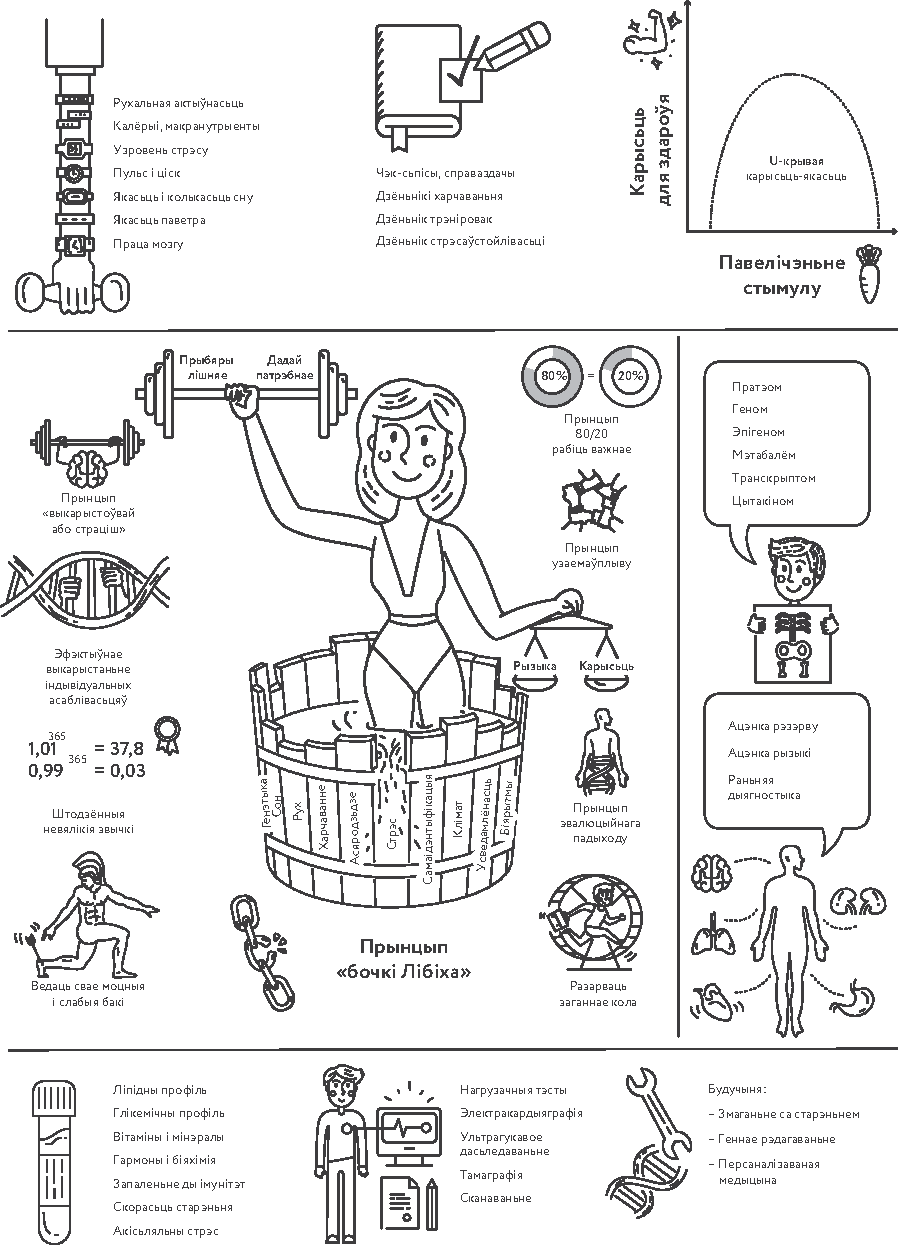
\includegraphics[width=\textwidth]{willpower/ch3/full.pdf}  
\end{figure*}
